\documentclass{article}
\usepackage{amsmath, amssymb, array, enumitem, fancyhdr, graphicx, hyperref,
libertine, multicol, multirow, nth, pgfplots, setspace, tikz, units, xcolor}
\hypersetup{
  colorlinks,
  citecolor=black,
  filecolor=black,
  linkcolor=black,
  urlcolor=black
}
\pgfplotsset{compat=1.11}
\usetikzlibrary{decorations.pathreplacing}
\usetikzlibrary{patterns}
\usetikzlibrary{shapes.multipart}
\usetikzlibrary{intersections}
\usepgfplotslibrary{fillbetween}
\usepackage[margin=1in]{geometry}
\usepackage[libertine]{newtxmath}
\onehalfspacing

\title{EC201 --- Summary of Each Topic}
\author{Christoph Walsh}
\begin{document}
\maketitle
\section{The Budget Constraint}
The \emph{budget constraint} is that you cannot spend more on goods $x_1$ and $x_2$ than your income $m$:
\[
  p_1x_1 + p_2x_2 \leq m
\]
The \emph{budget line} is when you exhaust your entire income:
\[
  p_1x_1 + p_2x_2 = m
\]
The vertical intercept of the budget line is at $\frac{m}{p_2}$ and the horizontal incercept is that $\frac{m}{p_1}$. Below is a graph of the budget line. The area below the budget line is the budget set, which is every bundle $\left( x_1,x_2 \right)$ the consumer can afford. The budget line represents the bundles the consumer can exactly afford (there is no money remaining).
\begin{center}
  \begin{tikzpicture}[baseline]
    \begin{axis}[axis equal,
                 ticks=none,
                 xmax=3,xmin=0,
                 ymin=-1,ymax=3,
                 xlabel=$x_1$,ylabel=$x_2$,
                 domain = 0:4,
                 axis x line = middle,
                 axis y line = middle,
                 width=10cm,
                 anchor=center]
      \addplot[samples=1000, restrict y to domain = 0:4] {2 - x};
      \draw (0, 2) node [left] {$\frac{m}{p_2}$};
      \draw (2, 0) node [below] {$\frac{m}{p_1}$};
      \draw (1.4, 0.8) node [right] {Slope: $-\frac{p_1}{p_2}$};
      \draw (0.8, 0.3) node {Budget set};
    \end{axis}
  \end{tikzpicture}
\end{center}
The slope of the budget line is $-\frac{p_1}{p_2}$. This is the \emph{opportunity cost} of consuming good 1. To consume one more unit of good 1 you need to give up $\frac{p_1}{p_2}$ units of good 2.
\begin{itemize}
  \item Changes in income result in parallel shifts of the budget line (both the vertical and horizontal intercepts change).
  \item Changes in one of the prices result in pivots of the budget line (only one of the intercepts change).
\end{itemize}

\section{Preferences}
$\left( x_1,x_2 \right)$ and $\left( y_1,y_2 \right)$ are two different consumption bundles that differ in the amounts of goods 1 and 2. Consumers rank consumption bundles $\left( x_1,x_2 \right)$ and $\left( y_1,y_2 \right)$.
\begin{itemize}
  \item If $\left( x_1,x_2 \right)\succ \left( y_1,y_2 \right)$, the consumer \emph{strictly prefers} $\left( x_1,x_2 \right)$ to $\left( y_1,y_2 \right)$. The consumer will always choose $\left( x_1,x_2 \right)$ over $\left( y_1,y_2 \right)$ if both are available.
  \item If $\left( x_1,x_2 \right)\sim \left( y_1,y_2 \right)$, the consumer is \emph{indifferent} between $\left( x_1,x_2 \right)$ and $\left( y_1,y_2 \right)$.
  \item If $\left( x_1,x_2 \right)\succeq \left( y_1,y_2 \right)$, the consumer \emph{weakly prefers} $\left( x_1,x_2 \right)$ to $\left( y_1,y_2 \right)$. If we observe a consumer choosing $\left( x_1,x_2 \right)$ over $\left( y_1,y_2 \right)$ if both were available, then we know that $\left( x_1,x_2 \right)\succeq \left( y_1,y_2 \right)$.
\end{itemize}
Some assumptions we often make about preferences:
\begin{description}
  \item[\textsc{Completeness:}] Either $\left( x_1,x_2 \right)\succeq \left( y_1,y_2 \right)$ or $\left( y_1,y_2 \right)\succeq \left( x_1,x_2 \right)$ or both.  You can always compare consumption bundles.
  \item[\textsc{Reflexivity:}] $\left( x_1,x_2 \right)\succeq \left( x_1,x_2 \right)$. A bundle is at least as good as itself.
  \item[\textsc{Transitivity:}] If $\left( x_1,x_2 \right)\succeq \left( y_1,y_2\right)$ and $\left( y_1,y_2 \right)\succeq \left( z_1,z_2\right)$, then $\left( x_1,x_2 \right)\succeq \left( z_1,z_2\right)$.
  \item[\textsc{Monotonicity:}] If either \begin{itemize} \item $x_1 \geq y_1$ and $x_2 > y_2$; or \item  $x_1 > y_1$ and $x_2 \geq y_2$
    \end{itemize}
    then $\left( x_1,x_2 \right)\succ \left( y_1,y_2 \right)$.

    Under monotonicity, a consumer prefers a bundle that has at least as much of all goods with strictly more of one of the goods.
  \item[\textsc{Convexity:}] Convexity means that consumers prefer variety.
    For all weights $t\in\left[ 0,1 \right]$, if $\left( x_1,x_2 \right)\sim \left( y_1,y_2 \right)$, then
    \[
    \left(tx_1+ \left( 1-t \right)y_1, tx_2 + \left( 1-t
    \right)y_2\right)\succeq \left( x_1,x_2 \right)
    \]
    Under convexity, a consumer would prefer the average of two extreme bundles to the extreme bundles themselves.
\end{description}
\subsubsection*{Indifference Curves:}
\begin{itemize}
  \item An \emph{indifference curve} joins all the bundles that are equally preferred to each other.
  \item Indifference curves cannot cross.
  \item Indifference curves for perfect substitutes are straight lines.
  \item Indifference curves for perfect complements are $L$-shaped.
\end{itemize}
\subsubsection*{The Marginal Rate of Substitution (MRS):}
\begin{itemize}
  \item The slope of the indifference curve at a point is called the \emph{marginal rate of substitution} (MRS).
  \item The MRS is how much of $x_2$ we need to give the consumer to keep them equally happy after taking away a small amount of $x_1$.
  \item In general the MRS is negative so we will often take the absolute value when interpreting it.
\end{itemize}
\begin{center}
  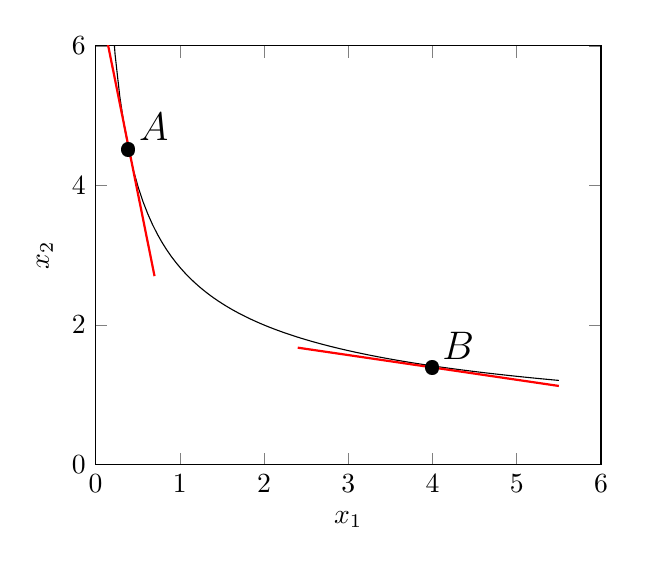
\begin{tikzpicture}[baseline]
    \begin{axis}[xmax=6,xmin=0,
                 ymin=0,ymax=6,
                 domain=0.01:5.5,
                 xlabel=$x_1$,ylabel=$x_2$,
                 width=8cm]
      \addplot[samples=100] {2^(3/2) / x^(0.5)};
      \addplot[red, thick, samples=100, domain=0.1:0.7] {6.9 - 6 * x};
      \draw (0.4, 4.5) node {\Large{\textbullet}};
      \draw (0.4, 4.5) node [above right] {\Large{$A$}};
      \addplot[red, thick, samples=100, domain=2.4:5.5] {2.10 - 0.177 * x};
      \draw (4, 1.365) node {\Large{\textbullet}};
      \draw (4, 1.365) node [above right] {\Large{$B$}};
    \end{axis}
  \end{tikzpicture}
\end{center}
\begin{itemize}
  \item At $A$ in the diagram above, the $MRS$ is very negative. You do not have very much $x_1$ and have a lot of $x_2$. You need to be given a lot of $x_2$ in order to be compensated for a loss in $x_1$.
  \item At $B$ in the diagram above, the $MRS$ is almost zero. You do have a lot of $x_1$ do not have very much $x_2$. You do not need to be given very much $x_2$ in order to be compensated for a loss in $x_1$.
\end{itemize}

\section{Utility}
A \emph{utility function}, $u$, is a way of assigning numbers to consumption bundles such that for every bundle where $\left( x_1,x_2 \right)\succ\left( y_1,y_2 \right)$ we have that $u\left( x_1,x_2 \right)>u\left( y_1,y_2 \right)$.
\begin{itemize}
  \item The actual numbers the utility function give don't matter, only insofar that the numbers rank bundles consistent with the preferences. This concept is called \emph{ordinal utility}.
  \item \emph{Cardinal utility} is when the actual numbers associated with different utilities do matter. In this case we can say things like ``bundle $\left( x_1,x_2 \right)$ is preferred \emph{twice as much} to bundle $\left( y_1,y_2 \right)$''.
  \item An indifference curve is all $x_1$ and $x_2$ such that $u\left( x_1,x_2 \right)=k$, where $k$ is some constant number. For example, if $u\left( x_1,x_2 \right)=x_1x_2$, then the indifference curve is $k=x_1x_2$, or $x_2=\frac{k}{x_1}$.
\end{itemize}
\subsubsection*{Common utility functions:}
\begin{center}
  \begin{tabular}{|l|l|}\hline
    Perfect substitutes & $u\left( x_1,x_2 \right)=ax_1 + bx_2$ \\\hline
    Perfect complements & $u\left( x_1,x_2 \right)=\min\left\{ ax_1,bx_2
    \right\}$ \\\hline
    Cobb-Douglas & $u\left( x_1,x_2 \right)=x_1^a x_2^b$ \\\hline
  \end{tabular}
\end{center}
\subsubsection*{Marginal Utility:}
\begin{itemize}
  \item The \emph{marginal utility} of a good is how much utility changes if we increase the amount of consumption of that good a tiny amount.
  \item It is the partial derivative of the utility function:
    \[
      MU_1 = \frac{\partial u\left( x_1,x_2 \right)}{\partial x_1} \;\;\;\;\;\;
      MU_2 = \frac{\partial u\left( x_1,x_2 \right)}{\partial x_2}
    \]
\end{itemize}
The marginal rate of substitution is equal to the (negative of the) ratio of marginal utilities:
\[
  MRS =- \frac{MU_1}{MU_2}=
    -\frac{\frac{\partial u\left( x_1,x_2\right)}{\partial x_1}}
          {\frac{\partial u\left( x_1,x_2\right)}{\partial x_2}}
\]
To see where this comes from, remember that the $MRS$ is the amount of $x_2$ we need to keep utility constant for a marginal change in $x_1$. So two small changes $dx_1$ and $dx_2$ that keeps utility constant satisfies:
\begin{equation*}
  du = \frac{\partial u\left( x_1,x_2 \right)}{\partial x_1}dx_1 +\frac{\partial u\left( x_1,x_2 \right)}{\partial x_2}dx_2  = 0
\end{equation*}
Solving yields:
\begin{equation*}
  \frac{dx_2}{dx_1}=MRS=
    -\frac{\frac{\partial u\left( x_1,x_2\right)}{\partial x_1}}
          {\frac{\partial u\left( x_1,x_2\right)}{\partial x_2}}=
  - \frac{MU_1}{MU_2}
\end{equation*}
\subsubsection*{Marginal Utility and \emph{MRS} Example with Cobb-Douglas Preferences:}
Suppose $u\left( x_1,x_2 \right)=x_1^ax_2^b$.
\begin{equation*}
  MU_1 = \frac{\partial u\left( x_1,x_2 \right)}{\partial x_1} = a x_1^{a-1}x_2^b
\end{equation*}
\begin{equation*}
  MU_2 = \frac{\partial u\left( x_1,x_2 \right)}{\partial x_2} = b x_1^{a}x_2^{b-1}
\end{equation*}
\begin{equation*}
  MRS = - \frac{MU_1}{MU_2}= - \frac{ax_1^{a-1}x_2^b}{bx_1^ax_2^{b-1}}=-\frac{a x_1^a x_1^{-1}x_2^b}{b x_1^a x_2^bx_2^{-1}}-\frac{ax_1^{-1}}{bx_2^{-1}} = -\frac{ax_2}{bx_1}
\end{equation*}

\section{Choice and Demand}
\subsubsection*{Optimal Choice}
\begin{itemize}
  \item If a consumer's preferences satisfy monotonicity, the optimal bundle will always lie on the budget line and not beneath it. The consumer will spend all of their money.
  \item If a consumer's preferences satisfy monotonicity, then indifference curves further away from the origin give higher utility. The consumer will want to choose a bundle that places them on the indifference curve the furthest away that is still affordable. This is the indifference curve that ``just touches'' the budget line.
  \item If preferences are smooth and the optimal choice is not on the boundary, the optimal bundle will be where the indifference curve is tangent to the budget line.
  \item The optimal consumption bundle for the consumer is not necessarily where the budget line is at a tangent to the indifference curve. For example:
    \begin{itemize}
      \item With perfect substitutes, if the prices are different you only buy the cheaper good. The optimal choice is at the boundary. The budget line will (in general) not line up with the tangent at the indifference curve.
      \item With perfect complements, you choose the bundle at the kink of the indifference curves. The tangent is not well defined at the kink.
    \end{itemize}
  \item With nonconvex preferences, it is possible that the point where the indifference curve is tangent to the budget line is suboptimal.
\end{itemize}
\subsubsection*{Demand Functions}
\begin{itemize}
  \item The \emph{demand function} is a function that relates the consumer's optimal choice to prices and incomes. We write demand functions for goods 1 and 2 as:
    \begin{equation*}
      x_1\left( p_1,p_2,m \right) \;\;\;\;\;\;\;\; x_2\left( p_1,p_2,m \right)
    \end{equation*}
  \item If we have perfect substitutes with a utility function $u\left( x_1,x_2 \right)=x_1+x_2$, the optimal choice is to buy the cheaper good. If the prices of the two goods are the same, buying either good or a combination of the two goods is optimal. The demand functions are then:
  \small
  \[
    \boxed{x_1\left( p_1,p_2,m \right)=
      \begin{cases}
        \frac{m}{p_1} & \text{ if } p_1<p_2 \\
        \text{any number between } 0 \text{ and } \frac{m}{p_1} &
        \text{ if } p_1 = p_2 \\
        0 & \text{ if } p_1>p_2 \\
      \end{cases}}
      \;\;\;\;
    \boxed{x_2\left( p_1,p_2,m \right)=
      \begin{cases}
        0 & \text{ if } p_1<p_2 \\
        \text{any number between } 0 \text{ and } \frac{m}{p_2} &
        \text{ if } p_1 = p_2 \\
        \frac{m}{p_2} & \text{ if } p_1>p_2 \\
      \end{cases}}
  \]
  \normalsize
\item If we have perfect complements with a utility function $u\left( x_1,x_2 \right)=\min\left\{ x_1,x_2 \right\}$, the optimal bundle will involve the same amount of goods 1 and 2. This is at the kink of the indifference curve that ``just touches'' the budget line. Setting $x_1=x_2$ and using this in the budget constraint:
  \begin{equation*}
    p_1x_1+p_2x_2= m \;\;\;\Longrightarrow \;\;\;
    p_1x_1 + p_2x_1 = m \;\;\; \Longrightarrow \;\;\;
    x_1\left( p_1+p_2 \right)=m \;\;\; \Longrightarrow \;\;\;
    x_1 = \frac{m}{p_1+p_2}
  \end{equation*}
  The demand functions for goods 1 and 2 are then:
  \[
    \boxed{x_1\left( p_1,p_2,m \right)= \frac{m}{p_1+p_2}}
      \;\;\;\;
    \boxed{x_2\left( p_1,p_2,m \right)= \frac{m}{p_1+p_2}}
  \]
  \item If we have well-behaved preferences (smooth, monotonic, convex) and if the optimal choice is interior (a nonzero amount of all goods) it is where the indifference curve is tangent to the budget line. The slope of the tangent of the indifference curve is the $MRS$. The slope of the budget line is $-\frac{p_1}{p_2}$. Therefore an interior solution to the consumer optimization problem with well-behaved preferences satisfies:
  \[
  \underbrace{MRS}_{\substack{\text{Slope of the} \\ \text{tangent of
  an} \\ \text{indifference curve} \\ \text{at a
  point}}}=\underbrace{-\frac{p_1}{p_2}}_{\substack{\text{Slope of the} \\
  \text{budget line}}}
  \]
  \item With monotonic preferences, the consumer will always exhaust their income when
  choosing the optimal consumption bundle. Therefore:
  \[
    p_1x_1 + p_2x_2 = m
  \]
  \item With these two optimality conditions, the demand functions $x_1\left(
  p_1,p_2,m\right)$ and $x_2\left( p_1,p_2,m \right)$ can be found by solving for
  $x_1$ and $x_2$ from these two equations:
  \[
    \boxed{\frac{\frac{\partial u\left( x_1,x_2\right)}{\partial x_1}}
    {\frac{\partial u\left( x_1,x_2\right)}{\partial x_2}} =
  \frac{p_1}{p_2}} \;\;\;\;
  \boxed{p_1x_1 + p_2x_2 = m}
  \]
\item With Cobb-Douglas preferences, $u\left( x_1,x_2 \right)=x_1^a x_2^b$, recall the $MRS$ was $-\frac{ax_2}{bx_1}$. Setting $MRS=-\frac{p_1}{p_2}$ and solving for $x_2$:
  \begin{equation*}
    \frac{ax_2}{bx_1}=\frac{p_1}{p_2} \;\;\;\Longrightarrow \;\;\;
    x_2=\frac{bp_1x_1}{ap_2}
  \end{equation*}
  We can use this in the budget line equation $p_1x_1 + p_2x_2=m$ to find the demand function for good 1:
  \begin{equation*}
    p_1x_1+p_2\left(\frac{bp_1x_1}{ap_2}\right) = m \;\;\;\Longrightarrow \;\;\;
    p_1x_1+\frac{bp_1x_1}{a} = m \;\;\;\Longrightarrow \;\;\;
    p_1x_1\left( 1+\frac{b}{a} \right) = m \;\;\;\Longrightarrow \;\;\;
    p_1x_1\frac{a+b}{a} = m \;\;\;\Longrightarrow \;\;\;
    x_1 = \frac{a}{a+b} \frac{m}{p_1}
  \end{equation*}
  We can use this in the expression for $x_2$ we found above to find the demand function for good 2:
  \begin{equation*}
    x_2=\frac{bp_1x_1}{ap_2} =\frac{bp_1\left( \frac{a}{a+b} \frac{m}{p_1} \right) }{ap_2}=\frac{b \left(\frac{a}{a+b}\right) m}{ap_2}=\frac{b \left(\frac{1}{a+b}\right) m}{p_2}=\frac{b}{a+b}\frac{m}{p_2}
  \end{equation*}
  The demand functions are then:
    \[
  x_1\left( p_1,p_2,m \right) = \frac{a}{a+b}\frac{m}{p_1} \;\;\;\;\;
  x_2\left( p_1,p_2,m \right) = \frac{b}{a+b}\frac{m}{p_2}
  \]
\end{itemize}
\subsubsection*{Income Changes}
\begin{itemize}
  \item A good is a \emph{normal good} if demand increases as income increases,
    i.e.~$\frac{dx_1}{dm}>0$.
  \item A good is an \emph{inferior good} if demand decreases as income increases,
    i.e.~$\frac{dx_1}{dm}<0$.
  \item The \emph{income offer curve} joins all the optimal consumption bundles
    for different levels of income $m$ at a fixed pair of prices $p_1$ and
    $p_2$.
  \item The \emph{Engel curve} plots the demand for a good against income, $m$,
    at a fixed pair of prices $p_1$ and $p_2$.
\end{itemize}
\subsubsection*{Own Price Changes}
\begin{itemize}
  \item If demand increases when the price of a good decreases, we call it an
    \emph{ordinary good}.
  \item If demand decreases when the price of a good decreases, we call it a
    \emph{Giffen good}.
  \item The \emph{price offer curve} for good 1 joins all the optimal consumption
    bundles for different $p_1$, holding $m$ and $p_2$ fixed.
  \item The \emph{demand curve} plots the demand for a good against its price,
    holding fixed income and the price of the other good.
\end{itemize}
\subsubsection*{Changes in the Price of the Other Good}
\begin{itemize}
  \item If the demand for good 1 goes up when the price of good 2 goes up, we
    say good 1 is a \emph{substitute} for good 2. This happens when
    $\frac{dx_1}{dp_2}>0$.
  \item If the demand for good 1 goes down when the price of good 2 goes up, we
    say good 1 is a \emph{complement} for good 2. This happens when
    $\frac{dx_1}{dp_2}<0$.
  \item If the demand for good 1 doesn't change when the price of good 2 goes
    up, good 1 is neither a substitute nor a complement to good 2. This
    happens when $\frac{dx_1}{dp_2}=0$.
\end{itemize}
\subsection*{Income and Substitution Effects}
\begin{itemize}
  \item When the price of a good changes, the optimal consumption bundle often changes. For example, if the price of good 1 decreases, you may buy more of good 1 and less of good 2.
  \item Part of this change is because the relative prices between the two goods have changed: you substitute towards good 1 because the price of good 1 decreased. This is the \emph{substitution effect}.
  \item The other part of this change is because with a lower price for good 1 you effectively have more income (your purchasing power increased). This is the \emph{income effect}.
\end{itemize}
To decompose the income and substitution effects, we consider what choice the consumer would have made had they experienced the relative price change but were at the original purchasing power. The change in the choice they make only facing the relative price change and not the change in purchasing power is the substitution effect. The remaining effect is the income effect.

The substitution effect is always such that the consumer buys more when the price falls and buys less when the price rises. To see why this is true, consider the example below. We are initially at $x^A$. Suppose we pivoted the budget line around $x^A$ (the blue line). This is what would happen if the price of good 1 fell and we brought the consumer's effective income back to the original bundle.  $x^C$ could never be optimal because $x^C$ was available before the pivot when $x^A$ was chosen while $x^A$ is still available after the pivot. Therefore the optimal choice after the pivot must be to the right of $x^A$. Therefore for price decreases the substitution effect is always nonnegative ($SE\geq 0$) and for price increases the substitution effect is always nonpositive ($SE\leq 0)$)

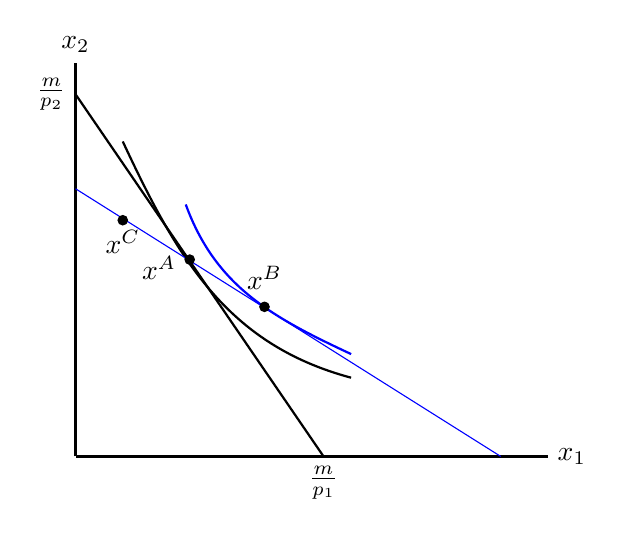
\begin{tikzpicture}[scale=1.0]
    \draw [thick] (0,0) -- (6,0);
    \draw [thick] (0,0) -- (0,5);
    \node [right] at (6,0) {$x_1$};
    \node [above] at (0,5) {$x_2$};
    \draw [thick] (0.6,4) to [out=295,in=165] (3.5,1);
    \draw [thick, blue] (1.4,3.2) to [out=290,in=155] (3.5,1.3);
    \draw [thick] (0,4.6) -- (3.15,0);
    \draw [blue] (0,3.4) -- (5.4,0);
    \node [above] at (2.4,2) {$x^B$};
    \draw[fill] (2.4,1.9) circle [radius =0.06];
    \node [left] at (1.4,2.4) {$x^A$};
    \draw[fill] (1.45,2.5) circle [radius =0.06];
    \draw[fill] (0.6,3.0) circle [radius =0.06];
    \node [below] at (0.6,3.0) {$x^C$};
    \node [left] at (0,4.6) {$\frac{m}{p_2}$};
    \node [below] at (3.15,0) {$\frac{m}{p_1}$};
  \end{tikzpicture}

  The income effect, on the other hand, can be positive or negative: it depends on the consumer's preferences. If good 1 normal, the income effect from a price decrease is positive. If good 1 is inferior, the income effect from a price decrease is negative.

\begin{multicols}{2}
\subsubsection*{Price decrease with a \emph{normal} good:}
We are initially consuming at $x^A$ with the black budget line. After the price of good 1 decreases (from $p_1$ to $p_1^\prime$), the budget line pivots outwards to $\frac{m}{p_1^\prime}$ (the blue budget line). The new consumption bundle is $x^C$. To decompose the income and substitution effects, we draw a new budget line which has the same slope as the new budget line ($-\frac{p_1^\prime}{p_2}$) but passes through the initial consumption plan $x^A$. This is the red dashed line. If this were the consumer's budget line, $x^B$ would be chosen which involves more of $x_1$. The substitution effect is changing from $x_1^A$ to $x_1^B$ and the income effect is changing from $x_1^B$ to $x_1^C$. The income and substitution effects are both positive when the price decreases.

\noindent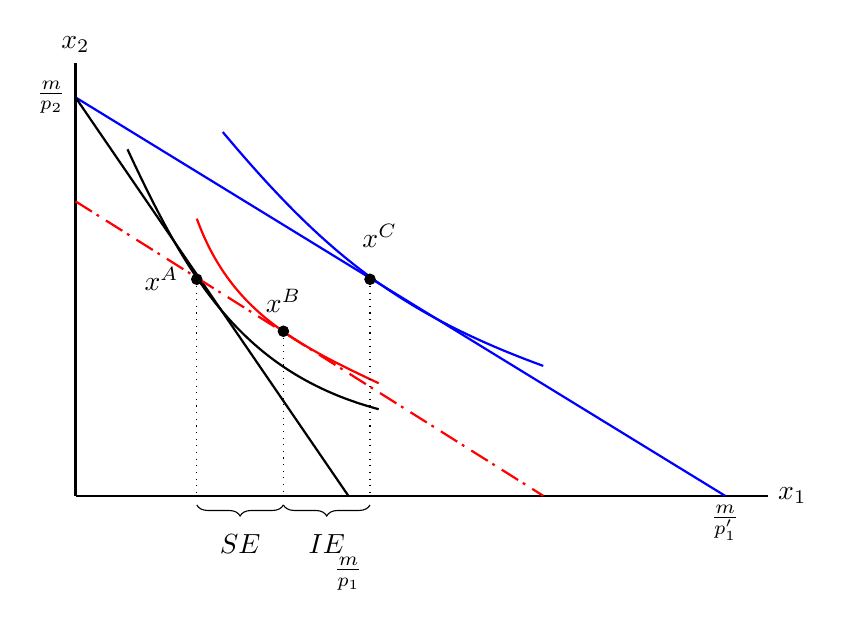
\begin{tikzpicture}[scale=1.1]
    \draw [thick] (0,0) -- (8,0);
    \draw [thick] (0,0) -- (0,5);
    \node [right] at (8,0) {$x_1$};
    \node [above] at (0,5) {$x_2$};
    \draw [thick, blue] (1.7,4.2) to [out=310,in=160] (5.4,1.5);
    \draw [thick] (0.6,4) to [out=295,in=165] (3.5,1);
    \draw [thick, red] (1.4,3.2) to [out=290,in=155] (3.5,1.3);
    \draw [thick, blue] (0,4.6) -- (7.5,0);
    \draw [thick] (0,4.6) -- (3.15,0);
    \draw[dotted](1.4,2.5)--(1.4,0);
    \draw[dotted](3.4,2.5)--(3.4,0);
    \draw [red,thick,dash pattern={on 7pt off 2pt on 1pt off 3pt}] (0,3.4) -- (5.4,0);
    \draw[dotted](2.4,1.9)--(2.4,0);
    \node [above] at (2.4,2) {$x^B$};
    \draw[fill] (2.4,1.9) circle [radius =0.06];
    \node [left] at (1.3,2.5) {$x^A$};
    \draw[fill] (1.4,2.5) circle [radius =0.06];
    \node [right] at (3.2,3) {$x^C$};
    \draw[fill] (3.4,2.5) circle [radius =0.06];
    \node [left] at (0,4.6) {$\frac{m}{p_2}$};
    \node [below] at (3.15,-0.6) {$\frac{m}{p_1}$};
    \node [below] at (7.5,0) {$\frac{m}{p_1^\prime}$};
    \draw [decorate,decoration={brace,amplitude=4pt, mirror},xshift=0pt,yshift=-3pt]
    (1.4,0) -- (2.4,0) node [black,midway,yshift=-.5cm] {$SE$};
    \draw [decorate,decoration={brace,amplitude=4pt, mirror},xshift=0pt,yshift=-3pt]
    (2.4,0) -- (3.4,0) node [black,midway,yshift=-.5cm] {$IE$};
  \end{tikzpicture}
\end{multicols}

\bigskip
\noindent\rule{\textwidth}{0.4pt}
\bigskip
\begin{multicols}{2}
  \subsubsection*{Price increase with a \emph{normal} good:}
  We are initially consuming at $x^A$ with the black budget line. After the price of good 1 increases (from $p_1$ to $p_1^\prime$), the budget line pivots inwards to $\frac{m}{p_1^\prime}$ (the blue budget line). The new consumption bundle is $x^C$. To decompose the income and substitution effects, we draw a new budget line which has the same slope as the new budget line ($-\frac{p_1^\prime}{p_2}$) but passes through the initial consumption plan $x^A$. This is the red dashed line. If this were the consumer's budget line, $x^B$ would be chosen which involves less of $x_1$. The substitution effect is changing from $x_1^A$ to $x_1^B$ and the income effect is changing from $x_1^B$ to $x_1^C$. The income and substitution effects are both negative when the price increases.

  \noindent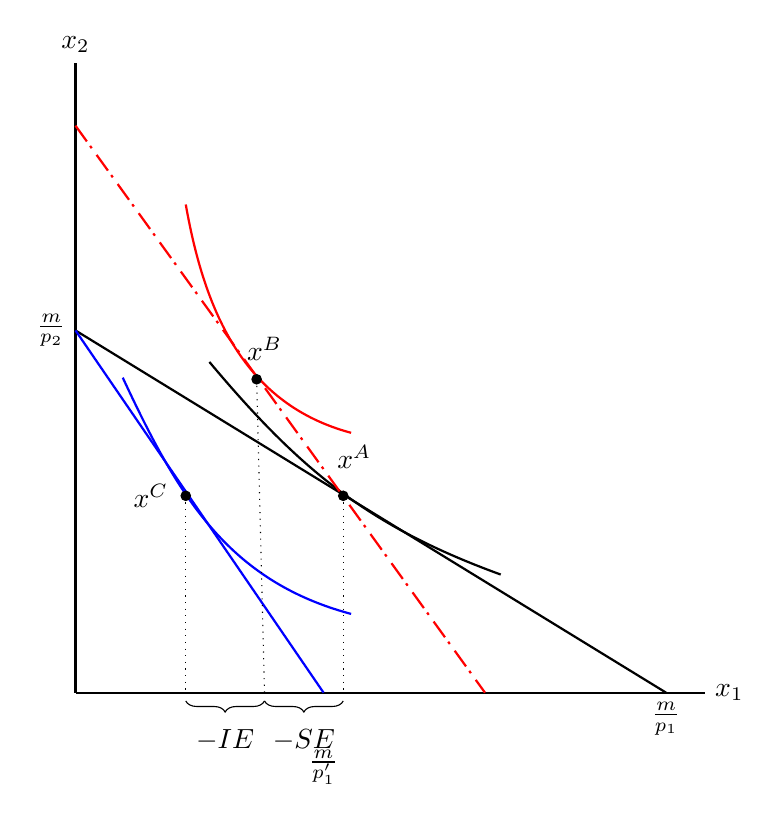
\begin{tikzpicture}[scale=1]
    \draw [thick] (0,0) -- (8,0);
    \draw [thick] (0,0) -- (0,8);
    \node [right] at (8,0) {$x_1$};
    \node [above] at (0,8) {$x_2$};
    \draw [thick, black] (1.7,4.2) to [out=310,in=160] (5.4,1.5);
    \draw [thick, blue] (0.6,4) to [out=295,in=165] (3.5,1);
    \draw [thick, red] (1.4,6.2) to [out=280,in=165] (3.5,3.3);
    \draw [thick] (0,4.6) -- (7.5,0);
    \draw [thick, blue] (0,4.6) -- (3.15,0);
    \draw[dotted](1.4,2.5)--(1.4,0);
    \draw[dotted](3.4,2.5)--(3.4,0);
    \draw [red,thick,dash pattern={on 7pt off 2pt on 1pt off 3pt}] (0,7.2) -- (5.2,0);
    \draw[dotted](2.3,3.98)--(2.4,0);
    \node [above] at (2.4,4.1) {$x^B$};
    \draw[fill] (2.3,3.98) circle [radius =0.06];
    \node [left] at (1.3,2.5) {$x^C$};
    \draw[fill] (1.4,2.5) circle [radius =0.06];
    \node [right] at (3.2,3) {$x^A$};
    \draw[fill] (3.4,2.5) circle [radius =0.06];
    \node [left] at (0,4.6) {$\frac{m}{p_2}$};
    \node [below] at (3.15,-0.6) {$\frac{m}{p_1^\prime}$};
    \node [below] at (7.5,0) {$\frac{m}{p_1}$};
    \draw [decorate,decoration={brace,amplitude=4pt, mirror},xshift=0pt,yshift=-3pt]
    (1.4,0) -- (2.4,0) node [black,midway,yshift=-.5cm] {$-IE$};
    \draw [decorate,decoration={brace,amplitude=4pt, mirror},xshift=0pt,yshift=-3pt]
    (2.4,0) -- (3.4,0) node [black,midway,yshift=-.5cm] {$-SE$};
  \end{tikzpicture}
\end{multicols}
\noindent\rule{\textwidth}{0.4pt}
\newpage
\begin{multicols}{2}
  \subsubsection*{Price decrease with an \emph{inferior} good (not Giffen):}
  We are initially consuming at $x^A$ with the black budget line. After the price of good 1 decreases (from $p_1$ to $p_1^\prime$), the budget line pivots outwards to $\frac{m}{p_1^\prime}$ (the blue budget line). The new consumption bundle is $x^C$. To decompose the income and substitution effects, we draw a new budget line which has the same slope as the new budget line ($-\frac{p_1^\prime}{p_2}$) but passes through the initial consumption plan $x^A$. This is the red dashed line. If this were the consumer's budget line, $x^B$ would be chosen which involves more of $x_1$. The substitution effect is changing from $x_1^A$ to $x_1^B$ and the income effect is changing from $x_1^B$ to $x_1^C$. The substitution effect is positive and the income effect is negative. The income effect, however, is not enough to outweigh the substitution effect: you still buy more of good 1 after the price decreases.

  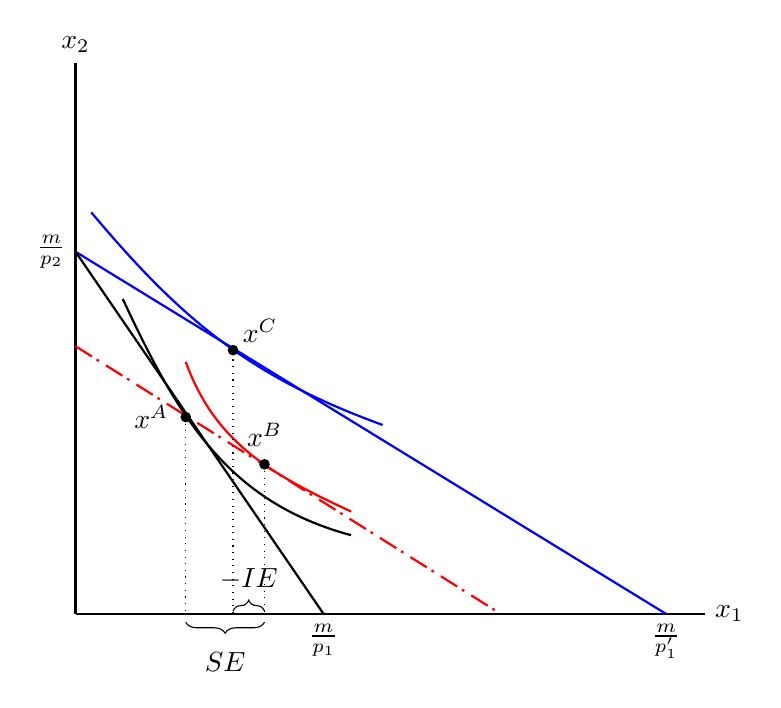
\begin{tikzpicture}[scale=1]
    \draw [thick] (0,0) -- (8,0);
    \draw [thick] (0,0) -- (0,7);
    \node [right] at (8,0) {$x_1$};
    \node [above] at (0,7) {$x_2$};
    \draw [thick, blue] (0.2,5.1) to [out=310,in=160] (3.9,2.4);
    \draw [thick] (0.6,4) to [out=295,in=165] (3.5,1);
    \draw [thick, red] (1.4,3.2) to [out=290,in=155] (3.5,1.3);
    \draw [thick, blue] (0,4.6) -- (7.5,0);
    \draw [thick] (0,4.6) -- (3.15,0);
    \draw[dotted](1.4,2.5)--(1.4,0);
    \draw[dotted](2.0,3.4)--(2.0,0);
    \draw [red,thick,dash pattern={on 7pt off 2pt on 1pt off 3pt}] (0,3.4) -- (5.4,0);
    \draw[dotted](2.4,1.9)--(2.4,0);
    \node [above] at (2.4,2) {$x^B$};
    \draw[fill] (2.4,1.9) circle [radius =0.06];
    \node [left] at (1.3,2.5) {$x^A$};
    \draw[fill] (1.4,2.5) circle [radius =0.06];
    \node [right] at (2.0,3.6) {$x^C$};
    \draw[fill] (2.0,3.35) circle [radius =0.06];
    \node [left] at (0,4.6) {$\frac{m}{p_2}$};
    \node [below] at (3.15,0) {$\frac{m}{p_1}$};
    \node [below] at (7.5,0) {$\frac{m}{p_1^\prime}$};
    \draw [decorate,decoration={brace,amplitude=4pt, mirror},xshift=0pt,yshift=-3pt]
    (1.4,0) -- (2.4,0) node [black,midway,yshift=-.5cm] {$SE$};
    \draw [decorate,decoration={brace,amplitude=4pt, mirror},xshift=0pt,yshift=1pt]
    (2.4,0) -- (2.0,0) node [black,midway,yshift=.4cm] {$-IE$};
  \end{tikzpicture}
\end{multicols}
\bigskip
\noindent\rule{\textwidth}{0.4pt}
\bigskip
\begin{multicols}{2}
  \subsubsection*{Price decrease with a Giffen good:}
  We are initially consuming at $x^A$ with the black budget line. After the price of good 1 decreases (from $p_1$ to $p_1^\prime$), the budget line pivots outwards to $\frac{m}{p_1^\prime}$ (the blue budget line). The new consumption bundle is $x^C$ (where $x_1^C<x_1^A$ as the good is Giffen). To decompose the income and substitution effects, we draw a new budget line which has the same slope as the new budget line ($-\frac{p_1^\prime}{p_2}$) but passes through the initial consumption plan $x^A$. This is the red dashed line. If this were the consumer's budget line, $x^B$ would be chosen which involves more of $x_1$. The substitution effect is changing from $x_1^A$ to $x_1^B$ and the income effect is changing from $x_1^B$ to $x_1^C$. The substitution effect is positive and the income effect is negative. The income effect is enough to outweigh the substitution effect such that you consume less of good 1 after the price falls.

  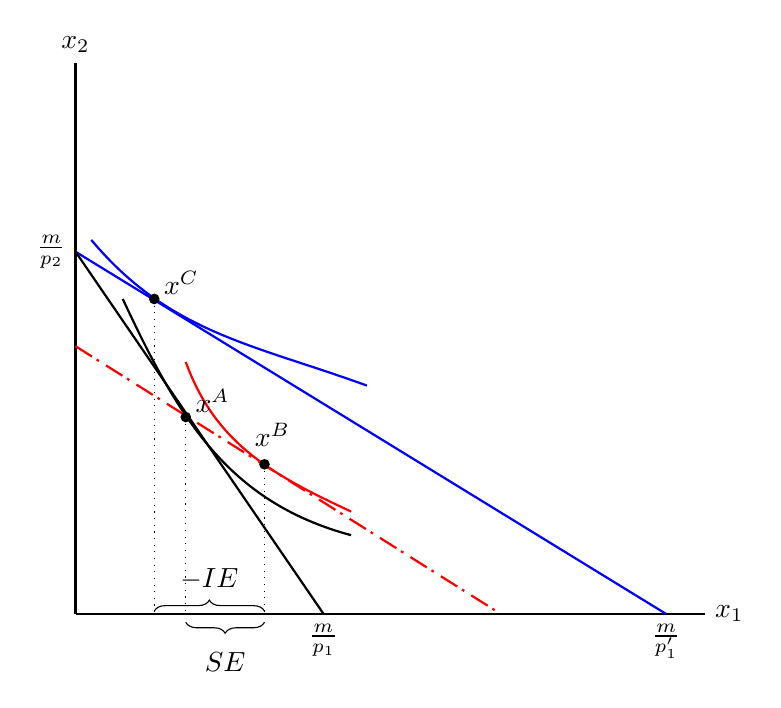
\begin{tikzpicture}[scale=1]
    \draw [thick] (0,0) -- (8,0);
    \draw [thick] (0,0) -- (0,7);
    \node [right] at (8,0) {$x_1$};
    \node [above] at (0,7) {$x_2$};
    \draw [thick, blue] (0.2,4.75) to [out=310,in=160] (3.7,2.9);
    \draw [thick] (0.6,4) to [out=295,in=165] (3.5,1);
    \draw [thick, red] (1.4,3.2) to [out=290,in=155] (3.5,1.3);
    \draw [thick, blue] (0,4.6) -- (7.5,0);
    \draw [thick] (0,4.6) -- (3.15,0);
    \draw[dotted](1.4,2.5)--(1.4,0);
    \draw[dotted](1.0,4.0)--(1.0,0);
    \draw [red,thick,dash pattern={on 7pt off 2pt on 1pt off 3pt}] (0,3.4) -- (5.4,0);
    \draw[dotted](2.4,1.9)--(2.4,0);
    \draw[fill] (1.4,2.5) circle [radius =0.06];
    \draw[fill] (1.0,4.0) circle [radius =0.06];
    \draw[fill] (2.4,1.9) circle [radius =0.06];
    \node [right] at (1.4,2.7) {$x^A$};
    \node [above] at (2.5,2) {$x^B$};
    \node [right] at (1.0,4.2) {$x^C$};
    \node [left] at (0,4.6) {$\frac{m}{p_2}$};
    \node [below] at (3.15,0) {$\frac{m}{p_1}$};
    \node [below] at (7.5,0) {$\frac{m}{p_1^\prime}$};
    \draw [decorate,decoration={brace,amplitude=4pt, mirror},xshift=0pt,yshift=-3pt]
    (1.4,0) -- (2.4,0) node [black,midway,yshift=-.5cm] {$SE$};
    \draw [decorate,decoration={brace,amplitude=4pt, mirror},xshift=0pt,yshift=1pt]
    (2.4,0) -- (1.0,0) node [black,midway,yshift=.4cm] {$-IE$};
  \end{tikzpicture}
\end{multicols}
\noindent\rule{\textwidth}{0.4pt}


\section{Intertemporal Choice}
This section is a variation on the consumer's choice problem. Instead of having two goods and deciding how much money to spend on each good, there is only one good and the consumer lives for two time periods and is deciding how much to borrow or save in the first period.

Call $c_1$ the consumption of the good in period 1 and $c_2$ the consumption of the good in period 2. Your income in period 1 is $m_1$ and your income in period 2 is $m_2$. We call $\left( m_1,m_2 \right)$ your \emph{endowment}. If you consume $c_1=m_1$ and $c_2=m_2$ (no borrowing or saving), we say you consume your endowment.

If there is no bank, you cannot borrow money and your savings do not earn any interest (you are stuffing cash in your mattress). If you save in period 1, your savings are $m_1-c_1$. Your consumption in period 2 is then $m_2+m_1-c$. You budget line is therefore
\begin{equation*}
  c_2 = \begin{cases} m_2 + m_1 - c_1 & \text{ if } m_1 - c_1 > 0 \text{ (you save)} \\ m_2 & \text{ if } m_1 - c_1 = 0 \text{ (you don't save)} \end{cases}
\end{equation*}
The budget line is:
\begin{center}
  \begin{tikzpicture}[scale=0.4]
    \draw [thick] (0,0) -- (11,0);
    \draw [thick] (0,0) -- (0,11);
    \node [right] at (11,0) {$c_1$};
    \node [above] at (0,11) {$c_2$};
    \draw [thick] (5,5) -- (0,10);
    \draw [thick] (5,5) -- (5,0);
    \draw[fill] (5,5) circle [radius =0.1];
    \draw[dotted,thick](5,5)--(0,5);
    \draw[dotted,thick](5,5)--(5,0);
    \node [below] at (5,0) {$m_1$};
    \node [left] at (0,5) {$m_2$};
    \node [left] at (0,10) {$m_1+m_2$};
  \end{tikzpicture}
\end{center}
Suppose now you can borrow or lend at an interest rate $r$ in period 1. Save $m_1-c_1$ in period 1 gives you $\left( 1+r \right)\left( m_1-c_1 \right)$ extra in period 2. Consumption in period 2 is therefore:
\begin{equation*}
  c_2 = m_2 + \left( 1+r \right)\left( m_1 - c_1 \right)
\end{equation*}
This is the budget constraint.
\begin{itemize}
  \item If $m_1 > c_1$, you saved in period 1 and earn interest.
  \item If $m_1 < c_1$ you borrowed in period 1 and you pay interest.
\end{itemize}
We can rearrange the budget constraint to:
\[
  c_2 = m_2 + \left( 1+r\right)\left( m_1-c_1 \right)
  \;\;\;\;\;\;\Longleftrightarrow \;\;\;\;\;\;
  \underbrace{c_1 + \frac{c_2}{1+r}}_{\substack{
    \text{Present value} \\ \text{of lifetime} \\ \text{consumption}}}
       =
  \underbrace{m_1 + \frac{m_2}{1+r}}_{\substack{
    \text{Present value} \\ \text{of lifetime} \\ \text{income}}}
\]
Comparing to our old budget constraint, this is like $p_1=1$, $p_2=\frac{1}{1+r}$ and $m=m_1 + \frac{m_2}{1+r}$.
\begin{center}
  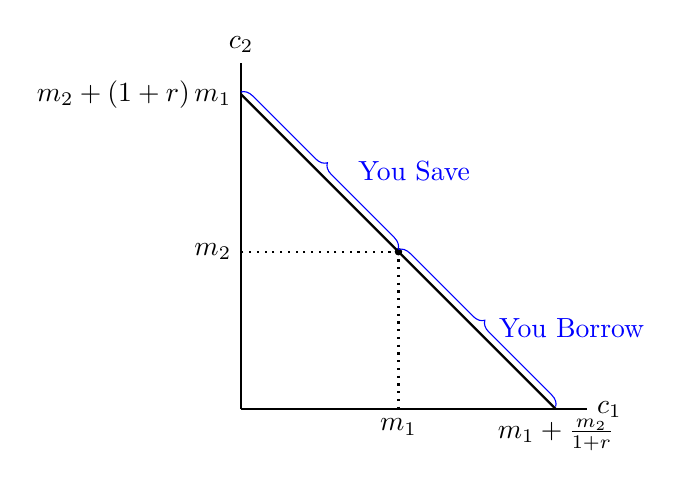
\begin{tikzpicture}[scale=0.4]
    \draw [thick] (0,0) -- (11,0);
    \draw [thick] (0,0) -- (0,11);
    \node [right] at (11,0) {$c_1$};
    \node [above] at (0,11) {$c_2$};
    \draw [thick] (10,0) -- (0,10);
    \draw[fill] (5,5) circle [radius =0.1];
    \draw[dotted,thick](5,5)--(0,5);
    \draw[dotted,thick](5,5)--(5,0);
    \node [below] at (5,0) {$m_1$};
    \node [left] at (0,5) {$m_2$};
    \node [left] at (0,10) {$m_2+\left( 1+r \right)m_1$};
    \node [below] at (10,0) {$m_1+\frac{m_2}{1+r}$};
    \draw [blue,decorate,decoration={brace,amplitude=4pt},xshift=0pt,yshift=2pt]
    (0,10) -- (5,5) node [blue,midway,xshift=1.2cm] {You Save};
    \draw [blue,decorate,decoration={brace,amplitude=4pt},xshift=0pt,yshift=2pt]
    (5,5) -- (10,0) node [blue,midway,xshift=1.2cm] {You Borrow};
  \end{tikzpicture}
\end{center}
An increase in the interest rate ($r\rightarrow r^\prime$) pivots the budget
line around the endowment
$\left( m_1,m_2 \right)$:
\begin{center}
  \begin{tikzpicture}[baseline]
    \begin{axis}[axis equal,
                 ticks=none,
                 xmax=3,xmin=0,
                 ymin=-1,ymax=5,
                 xlabel=$c_1$,ylabel=$c_2$,
                 domain = 0:4,
                 axis x line = middle,
                 axis y line = middle,
                 width=10cm,
                 anchor=center]
      \addplot[samples=1000, restrict y to domain = 0:4] {2 - x};
      \addplot[dashed, magenta, samples=50, restrict y to domain = 0:4] {4 -
      4 * x};
      \draw (0, 2) node [left] {\scriptsize{$\left( 1+r \right)m_1+m_2$}};
      \draw (0, 4) node [red, left] {\scriptsize{$\left( 1+r^\prime
      \right)m_1+m_2$}};
      \draw (1, 0) node [red, below]
      {\scriptsize{$m_1+\frac{m_2}{1+r^\prime}$}};
      \draw (2, 0) node [below] {\scriptsize{$\;\;\;m_1+\frac{m_2}{1+r}$}};
      \draw (0.4, 3) node [red, right] {Slope: $-\left( 1+r^\prime \right)$};
      \draw (1.4, 0.8) node [right] {Slope: $-\left( 1+r \right)$};
      \draw (0.67, 1.32) node [blue] {\textbullet};
      \draw (1.4, 1.4) node [blue] {$\left( m_1,m_2 \right)$};
    \end{axis}
  \end{tikzpicture}
\end{center}
\begin{itemize}
  \item If you are a \emph{lender-type} person, you are made better off by an increase in the interest rate.
  \item If you are a \emph{borrower-type} person, you are made worse off by an increase in the interest rate.
\end{itemize}
\subsubsection*{Inflation}
With an inflation rate $\pi$ the budget constraint becomes:
\[
  c_2 = m_2 + \frac{1+r}{1+\pi}\left( m_1-c_1 \right)
\]
The real interest rate $\rho$ is defined by:
\[
  1+\rho = \frac{1+r}{1+\pi}
\]
If the inflation rate isn't too high, we can use the approximation:
$\rho\approx r-\pi$.
\subsubsection*{Valuing income streams}
\begin{itemize}
  \item  The present value of income is all that matters for your intertemporal budget constraint as long as you are able to borrow and lend at the same interest rate: it doesn't matter if you get all your income in period 1 or 2 as long as the present value of income is the same.
  \item The present value of an income stream that pays $x_1$ in period 1 and $x_2$ in period 2 is $PV=x_1 + \frac{x_2}{1+r}$.
  \item The present value of an income stream that pays $x$ forever (starting in period 2) is:
    \[ PV=\frac{x}{1+r}+\frac{x}{\left( 1+r \right)^2}+\frac{x}{\left( 1+r \right)^3} +\frac{x}{\left( 1+r \right)^4}+\dots=\frac{x}{r} \]
\end{itemize}

\section{Uncertainty}
This section is another variation on the consumption problem. First we had two goods and the consumer was deciding how much to consume of each good given their budget constraint. Then we had one good and two time periods and the consumer was deciding how much to borrow or save given their income stream and the interest rate. In this section, there will be different states of the world that occur with different possibilities. The consumer is deciding how much insurance to buy to smooth consumption across those states.

\subsubsection*{Insurance}
You have an asset worth $A$. In state 1 the asset receives a loss in value $L$. For example, the asset is a car and state 1 is a car crash which results in damage worth $L$ to the car. In state 2, the asset retains its value $A$ (there is no car crash). The probability of state 1 is $\pi_1$ and the probability of state 2 is $\pi_2$.

Without insurance your consumption in state 1 is $c_1=A-L$ and your consumption in state 2 is $c_2=A$. You can purchase insurance that will pay $K$ if the loss occurs for $\gamma K$. $\gamma$ can be interpreted as the cost per dollar of insurance. To fully insure, you set $K=L$. In this case, you get $A-\gamma L$ in both states, where $\gamma L$ is the cost of insurance. This is shown graphically below.

\begin{center}
  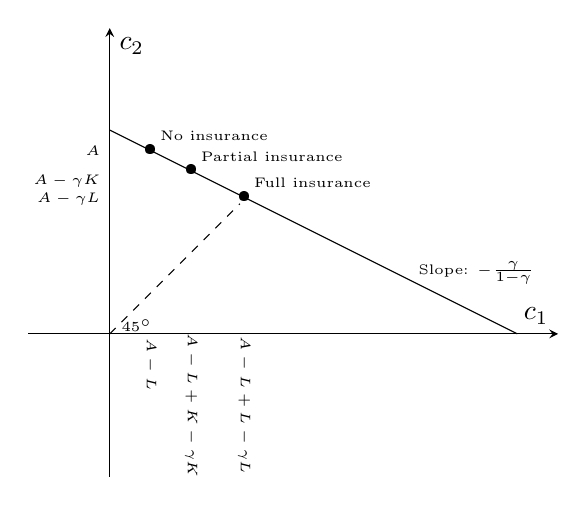
\begin{tikzpicture}[baseline]
    \begin{axis}[ticks=none,
                 axis equal image,
                 xmax=2.2,xmin=-0.4,
                 ymin=-0.7,ymax=1.5,
                 xlabel=$c_1$,ylabel=$c_2$,
                 domain = 0:2,
                 axis x line = middle,
                 axis y line = middle,
                 anchor=center]
      \addplot[samples=1000, restrict y to domain = 0:4] {1 - 0.5 *x};
      %% No insurance %%
      \draw (0.2, 0.9) node {\textbullet};
      \draw (0.2, 0.9) node [above right] {\tiny{No insurance}};
      \draw (0, 0.9) node [left] {\tiny{$A$}};
      \draw (0.2, -0.15) node [rotate=-90] {\tiny{$A-L$}};
      %% Full insurance %%
      \draw (0.66, 0.67) node {\textbullet};
      \draw (0.66, 0.67) node [above right] {\tiny{Full insurance}};
      \draw (0, 0.66) node [left] {\tiny{$A - \gamma L$}};
      \draw (0.66, -0.35) node [rotate=-90] {\tiny{$A - L + L - \gamma L$}};
      %% Partial insurance %%
      \draw (0.4, 0.8) node {\textbullet};
      \draw (0.4, 0.8) node [above right] {\tiny{Partial insurance}};
      \draw (0, 0.75) node [left] {\tiny{$A-\gamma K$}};
      \draw (0.4, -0.35) node [rotate=-90] {\tiny{$A-L+K-\gamma K$}};
      %% 45-degree line %%
      \addplot[samples=1000, dashed, restrict y to domain = 0:0.64] {x};
      \draw (0.01, 0.04) node [right] {\tiny{$45^\circ$}};
      %% Slope label %%
      \draw (1.8, 0.3) node {\tiny{Slope: $-\frac{\gamma}{1-\gamma}$}};
    \end{axis}
  \end{tikzpicture}
\end{center}
\subsubsection*{Expected Utility}
How much a person will value consumption in a world with risk state depends on both the consumption in each state and the probability that each state will occur. Therefore the utility function will be a function of both the consumption levels and the probabilities: $u\left( c_1,c_2,\pi_1,\pi_2 \right)$. One way to write this utility function is the weighted average of utility in each state, where the weights are the probabilities that those states occur. This is called \emph{expected utility}:
\begin{equation*}
  u\left( c_1,c_2,\pi_1,\pi_2 \right)= \pi_1 v\left( c_1 \right) + \pi_2 v\left( c_2 \right)
\end{equation*}
$v$ is a function which gives the utility of consumption within a state. For example, it could be $v\left( x \right)=\sqrt{x}$. Expected utility would then be:
\begin{equation*}
  u\left( c_1,c_2,\pi_1,\pi_2 \right)= \pi_1 \sqrt{c_1} + \pi_2 \sqrt{c_2}
\end{equation*}
In this context, the marginal rate of substitution of consumption between both states is:
\[
  MRS = -\frac{\frac{\partial u\left(c_1,c_2,\pi_1,\pi_2\right)}{\partial c_1}}
              {\frac{\partial u\left(c_1,c_2,\pi_1,\pi_2\right)}{\partial c_2}}
  = -\frac{\pi_1\frac{\partial v\left(c_1\right)}{\partial c_1}}
          {\pi_2\frac{\partial v\left(c_2\right)}{\partial c_2}}
\]
\subsubsection*{Preferences for Risk}
Suppose you have \$10 and someone offers you the following gamble based on a coin toss. If the coin lands on heads, you will give them \$5. If the coin lands on tails, they will give you \$5. Your expected value of wealth from not taking this gamble is \$10 (you just keep your money). Your expected value from taking the gamble is:
\begin{equation*}
  \pi_1 c_1 + \pi_2 c_2 = 0.5 \times \$15 + 0.5 \times \$5 = \$10
\end{equation*}
The ``sure thing'' is \$10 and the expected value of the gamble is \$10. Whether or not you might take this gamble depends on your preferences for risk. There are three main different types of preferences for risk:
\begin{itemize}
  \item \emph{Risk-averse} consumers prefer ``sure things'' to gambles that have the same expected value. Their utility functions are \emph{concave}.
  \item \emph{Risk-neutral} consumers are indifferent between ``sure things'' and gambles that have the same expected value. Their utility functions are \emph{linear}.
  \item \emph{Risk-loving} consumers prefer gambles to ``sure things'' that have the same expected value. Their utility functions are \emph{convex}.
\end{itemize}
Going back to the coin toss example:
\begin{itemize}
  \item An example of a risk-averse utility function is $v\left( x \right)=\sqrt{x}$. The expected utility from the ``sure thing'' is $0.5\times\sqrt{10} + 0.5\times\sqrt{10}=\sqrt{10}\approx 3.16$. The expected utility from the gamble is $0.5\times \sqrt{5} + 0.5\times \sqrt{15}\approx 3.05$. The risk-averse consumer prefers the sure thing.
  \item An example of a risk-neutral utility function is $v\left( x \right)=x$. The expected utility from the ``sure thing'' is $10$. The expected utility from the gamble is $0.5\times 5 + 0.5 \times 15 = 10$. The risk-neutral consumer is indifferent between the ``sure thing'' and the gamble.
  \item An example of a risk-loving utility function is $v\left( x \right)=x^2$. The expected utility from the ``sure thing'' is $10^2=100$. The expected utility from the gamble is $0.5\times 5^2 + 0.5 \times 15^2 = 125$. The risk-loving consumer prefers the gamble to the ``sure thing''.
\end{itemize}
\subsubsection*{Optimal Amount of Insurance}
If the consumer is risk-averse, the optimal amount of insurance is where the marginal rate of substitution is equal to the slope of the budget line. Here, the slope of the budget line is $-\frac{\gamma}{1-\gamma}$ so:
\begin{equation*}
  \frac{\pi_1\frac{\partial v\left(c_1\right)}{\partial c_1}}
          {\pi_2\frac{\partial v\left(c_2\right)}{\partial c_2}}
       =\frac{\gamma}{1-\gamma}
\end{equation*}
If we assume the insurance company has no costs other than paying out when accidents occur, the profit for the insurance company is $Profits =\gamma K - \pi_1 K$. In a competitive insurance market, the insurance company breaks even ($Profits=0$) so $\gamma = \pi_1$. When the insurance premium is the same as the probability of the loss occurring, we call this an \emph{actuarially fair} premium. With an actuarially fair premium, the probabilities and $\gamma$ terms cancel so:
\begin{equation*}
  \frac{\partial v\left(c_1\right)}{\partial c_1}=
  \frac{\partial v\left(c_2\right)}{\partial c_2}
\end{equation*}
In this case\footnote{This requires $\frac{\partial v}{\partial c}$ to be a strictly monotonic function. Since the consumer is risk averse, we know $v$ is concave, which ensures that $\frac{\partial v}{\partial c}$ is a strictly decreasing function.}, $ \frac{\partial v\left(c_1\right)}{\partial c_1}= \frac{\partial v\left(c_2\right)}{\partial c_2}$ implies that $c_1=c_2$.
Therefore if consumers are risk averse and premiums are \emph{actuarially fair}, then they will optimally choose to fully insure.

\section{Technology}
\begin{itemize}
  \item A firm's \emph{production function} $f$ shows how factors of production
    (inputs) are converted into output: $y=f\left( x_1,x_2 \right)$.
  \item An \emph{isoquant} shows the various combinations of inputs $\left(
    x_1,x_2 \right)$ that will yield the same amount of output $y$.
  \item The \emph{monotonicty} assumption is that more inputs will give more
    output.
  \item The \emph{convexity} assumption is that the average of two input
    combinations $\left( x_1,x_2 \right)$ and $\left( x_1^\prime, x_2^\prime
    \right)$ will yield at least as much output.
  \item The \emph{marginal product} of a factor is how much output changes in
    response to a marginal increase in the factor, holding the other factors of
    production fixed:
    \[
      MP_1 = \frac{\partial f\left( x_1,x_2 \right)}{\partial x_1}
      \;\;\;\;\;\;\;\;\;\;\;\;\;
      MP_2 = \frac{\partial f\left( x_1,x_2 \right)}{\partial x_2}
    \]
  \item The technical rate of substitution ($TRS$) is how much of factor 2 we
    need to produce the same amount of output $y$ if we reduce factor 1 a
    marginal amount:
    \[
      TRS = - \frac{MP_1}{MP_2} =
      - \frac{\frac{\partial f\left( x_1,x_2 \right)}{\partial
      x_1}}{\frac{\partial f\left( x_1,x_2 \right)}{\partial x_2}}
    \]
    The $TRS$ is the slope of an isoquant at a point.
  \item The \emph{law of diminishing marginal product} is that the marginal
    product of a factor will fall as we increase the use of that factor, while
    holding other factors fixed.
\end{itemize}
\subsubsection*{Returns to Scale}
For some number $t>1$:
\begin{itemize}
  \item If $tf\left( x_1,x_2 \right) = f\left( tx_1,tx_2 \right)$, then $f$
    exhibits constant returns to scale (CRS).
  \item If $tf\left( x_1,x_2 \right) < f\left( tx_1,tx_2 \right)$, then $f$
    exhibits increasing returns to scale (IRS).
  \item If $tf\left( x_1,x_2 \right) > f\left( tx_1,tx_2 \right)$, then $f$
    exhibits decreasing returns to scale (DRS).
\end{itemize}
For Cobb-Douglas technology, $f\left( x_1,x_2 \right)=x_1^ax_2^b$, scaling each
input by $t$ yields: $f\left( tx_1,tx_2 \right)= \left( tx_1 \right)^a\left(
tx_2\right)^b=t^{a+b}f\left( x_1,x_2 \right)$. If $a+b=1$, there is CRS. If
$a+b<1$, there is DRS. If $a+b>1$, there is IRS.

\section{Profit Maximization}
\subsubsection*{Short-Run Profit Maximization}
Suppose the production function is $y=f\left( x_1,x_2 \right)$, the price of output is $p$ and the prices of each input/factor are $w_1$ and $w_2$. The firm is competitive and therefore has no control over input and output prices.  Factor 2 is fixed in the short run, $x_2=\bar{x}_2$. The firm's maximization problem is:
\[
  \underset{x_1}{\max}\; pf\left( x_1,\bar{x}_2 \right) - w_1x_1 - w_2\bar{x}_2
\]
The firm chooses $x_1$ to maximize profits. This is done by taking the derivative of the above with respect to $x_1$ and setting the derivative equal to zero:
\[
  p\underbrace{\frac{\partial f\left( x_1,\bar{x}_2 \right)}{\partial x_1}}_{=MP_1} - w_1 =0
\]
This gives:
\[
  \underbrace{pMP_1}_{\substack{\text{Value of the} \\ \text{marginal product}
  \\ \text{of factor 1}}}
  = \underbrace{w_1}_{\substack{\text{Price of} \\ \text{factor 1}}}
\]
\subsubsection*{Long-Run Profit Maximization}
In the long run, the firm chooses both $x_1$ and $x_2$:
\[
  \underset{x_1, x_2}{\max}\; pf\left( x_1,x_2 \right) - w_1x_1 - w_2x_2
\]
The optimality conditions are:
\begin{align*}
  p\underbrace{\frac{\partial f\left( x_1,x_2 \right)}{\partial x_1}}_{=MP_1} -
  w_1 &=0 \\
  p\underbrace{\frac{\partial f\left( x_1,x_2 \right)}{\partial x_2}}_{=MP_2} -
  w_2 &=0
\end{align*}
These equations give the factor demand curves $x_1\left( p,w_1,w_2 \right)$ and $x_2\left( p,w_1,w_2 \right)$. The factor demand curves give the optimal choice of inputs given the output price and the input prices.
% \par\noindent\emph{Cobb-Douglas Example:}
% \begin{equation*}
%   \underset{\left\{x_1,x_2\right\}}{\max}\;\;px_1^ax_2^b - w_1x_1 -w_2x_2
% \end{equation*}
% Taking the partial derivatives with respect to $x_1$ and $x_2$ and setting them equal to zero:
% \begin{align}
%   p a x_1^{a-1}x_2^b - w_1 &= 0 \\
%   p b x_1^{a}x_2^{b-1} - w_2 &= 0
% \end{align}
% Multiplying (1) across by $x_1$ and (2) across by $x_2$:
% \begin{align*}
%   p a \underbrace{x_1^{a}x_2^b}_{=y} - w_1x_1 &= 0 \\
%   p b \underbrace{x_1^{a}x_2^{b}}_{=y} - w_2 x_2&= 0
% \end{align*}
% Solving each for $x_1$ and $x_2$:
% \begin{align*}
%   x_1 = \frac{pay}{w_1} \\
%   x_2 = \frac{pby}{w_2}
% \end{align*}

\subsubsection*{Profit Maximization and Returns to Scale}
Suppose there was some choice of $x_1$ and $x_2$ that the firm earned a profit:
\[
pf\left( x_1,x_2 \right) - w_1x_1 - w_2x_2 > 0
\]
If the production function exhibited constant returns to scale and we increased production by a factor of $t$:
\[
pf\left( tx_1,tx_2 \right) - w_1tx_1 - w_2tx_2 =
ptf\left( x_1,x_2 \right) - w_1tx_1 - w_2tx_2 =
t\underbrace{\left[pf\left( x_1,x_2 \right) - w_1x_1 - w_2x_2\right]}_{>0}
\]
The firm could choose $t$ to be infinitely large and earn infinite profits. Therefore when we observe constant returns to scale, there are zero profits in equilibrium.

\section{Cost Curves}
\begin{itemize}
  \item The cost function $c\left( y \right)$ gives the minimum cost of producing output level $y$.
  \item Costs can be decomposed into \emph{variable costs}, denoted by $c_v\left( y \right)$, and \emph{fixed costs}, denoted by $FC$:
    \[c\left( y \right)= c_v\left( y \right)+FC\]
  \item \emph{Variable costs} are costs that vary with output. If no output is produced, the variable costs are zero.
  \item \emph{Fixed costs} are costs that do not depend on output. Fixed costs are paid even when the firm does not produce any output. If a firm does not produce any output, total costs equal fixed costs.
  \item An example cost function is $c\left( y \right)=y^2+1$. Here the fixed cost is $FC=1$ (the constant) and the variable cost is $c_v\left( y \right)=y^2$.
  \item The \emph{average cost function} measures cost per unit of output:
  \[AC\left(
y \right)=\frac{c\left( y \right)}{y}\]
  \item In the example cost function $c\left( y \right)=y^2+1$, the average cost is $AC\left( y \right)=\frac{y^2+1}{y}=y+\frac{1}{y}$.
  \item We also have average variable costs, $AVC\left( y \right)$, and average fixed costs, $AFC\left( y \right)$:
    \[
    AC\left( y \right) = \frac{c\left( y \right)}{y}=\frac{c_v\left( y
    \right)+FC}{y} = \frac{c_v\left( y \right)}{y} + \frac{FC}{y} = AVC\left(
    y \right) + AFC\left( y \right)
    \]
    Notice that while fixed costs do not depend on $y$, average fixed costs do depend on $y$. Average fixed costs always fall as $y$ increases.
  \item In the example cost function $c\left( y \right)=y^2+1$,  the average variable cost is $AVC\left( y \right)=\frac{y^2}{y}=y$ and the average fixed cost is $AFC\left( y \right)=\frac{1}{y}$.
  \item Average variable costs are always below average costs due to the presence of fixed costs (unless fixed costs are zero). The difference between $AC\left( y \right)$ and $AVC\left( y \right)$ falls as $y$ gets large because $AFC\left( y \right)$ gets smaller.
\end{itemize}
\begin{center}
  \begin{tikzpicture}[scale=0.7]
    \begin{axis}[ticks=none,
                 xmax=10,xmin=-2,
                 ymin=-15,ymax=100,
                 axis lines=middle,
                 width=13cm,
               xlabel=$y$,ylabel=\hspace{-8mm}$\$$]
      \addplot[thick, samples=100][domain=0:10] {15/x + 50-8*x+x^2};
      \addplot[thick, blue, samples=100][domain=0:10] {50-8*x+x^2};
      \draw (8, 60) node {$AC$};
      \draw[blue] (9, 50) node {$AVC$};
    \end{axis}
  \end{tikzpicture}
\end{center}

\begin{itemize}
  \item The \emph{marginal cost} measures the change in costs for a small change in output.
  \item If we change output by one unit, the marginal cost is $c\left( y \right)-c\left( y-1 \right)$.
  \item For small changes, the marginal cost is the derivative of the cost function with respect to output: \[MC\left( y \right)=\frac{dc\left( y \right)}{dy}\]
  \item In the example cost function $c\left( y \right)=y^2+1$, the marginal cost is $\frac{dc\left( y \right)}{dy}=2y$.
  \item Since fixed costs do not vary with output, the marginal cost curve is also the derivative of the variable cost curve:
    \begin{equation*}
      c\left( y \right)=c_v\left( y \right)+FC
    \end{equation*}
    Taking derivatives of both sides:
    \begin{equation*}
      \frac{dc\left( y \right)}{dy} =\frac{dc_v\left( y \right)}{dy} +\underbrace{\frac{d\left( FC \right)}{dy}}_{=0} = \frac{dc_v\left( y \right)}{dy}
    \end{equation*}
    Therefore $MC\left( y \right)=\frac{dc\left( y \right)}{dy}=\frac{dc_v\left( y \right)}{dy}$
\end{itemize}
\subsubsection*{Relationship between Marginal Cost, Average Variable Cost and Average Cost}
\begin{itemize}
  \item If the average variable cost function is decreasing, then then marginal cost must be less than the average variable cost.
    \begin{itemize}
      \item Suppose you measured the height of everyone in the room and took the average height. Then someone entered the room who was shorter than the average. If you take the average again, the average would be lower as the new person lowered the average.
      \item To see this mathematically, we can use the quotient rule to find the derivative of the average variable cost function:
        \begin{equation*}
          \frac{dAVC\left( y \right)}{dy}= \frac{d\left(\frac{c_v\left( y \right)}{y}  \right)}{dy} = \frac{yc_v^{\prime}\left( y \right)-c_v\left( y \right)}{y^2}
        \end{equation*}
        If the average variable cost is decreasing, then $\frac{dAVC\left( y \right)}{dy}<0$. Therefore:
        \begin{align*}
         \frac{yc_v^{\prime}\left( y \right)-c_v\left( y \right)}{y^2} &< 0\\
         yc_v^{\prime}\left( y \right)-c_v\left( y \right) &< 0\\
         yc_v^{\prime}\left( y \right)&< c_v\left( y \right)\\
         \underbrace{c_v^{\prime}\left( y \right)}_{MC\left( y \right)}&< \underbrace{\frac{c_v\left( y \right)}{y}}_{=AVC\left( y \right)}\\
        \end{align*}
    \end{itemize}
  \item Similarly, if the average variable cost function is increasing, then the marginal cost function must be greater than the average variable cost.
  \item The marginal cost curve is equal to the average variable cost curve when the average variable cost is at its minimum, i.e.~when $\frac{dAVC\left( y \right)}{dy}=0$. We can use the same steps as above to see this:
        \begin{align*}
        \frac{dAVC\left( y \right)}{dy} &= 0 \\
         \frac{yc_v^{\prime}\left( y \right)-c_v\left( y \right)}{y^2} &= 0\\
         yc_v^{\prime}\left( y \right)-c_v\left( y \right) &= 0\\
         yc_v^{\prime}\left( y \right)&= c_v\left( y \right)\\
         \underbrace{c_v^{\prime}\left( y \right)}_{MC\left( y \right)}&= \underbrace{\frac{c_v\left( y \right)}{y}}_{=AVC\left( y \right)}\\
        \end{align*}
  \item We can also follow the almost the same steps to show that the marginal cost curve is equal to average total cost at its minimum.
  \item These relationships between marginal cost, average cost and average variable cost can be shown graphically as follows:
\end{itemize}
\begin{center}
  \begin{tikzpicture}[scale=0.7]
    \begin{axis}[ticks=none,
                 xmax=10,xmin=-2,
                 ymin=-15,ymax=100,
                 axis lines=middle,
                 width=13cm,
               xlabel=$y$,ylabel=\hspace{-8mm}$\$$]
      \addplot[thick, samples=100][domain=0:10] {15/x + 50-8*x+x^2};
      \addplot[thick, blue, samples=100][domain=0:10] {50-8*x+x^2};
      \addplot[thick, red, samples=100][domain=0:10] {50-16*x+3*x^2};
      \draw (8, 60) node {$AC$};
      \draw[blue] (9, 50) node {$AVC$};
      \draw[red] (7.5, 80) node {$MC$};
    \end{axis}
  \end{tikzpicture}
\end{center}
\subsubsection*{Relationship between Marginal Cost, Average Variable Cost and Average Cost}
\begin{itemize}
  \item The variable cost of producing $y$ is the sum of marginal costs up to
    $y$.
  \item If output $y$ is discrete, we can see this as follows:
    \begin{align*}
      c_v\left( y \right)&=c_v\left( 0 \right) - c_v\left( 0 \right) +
      c_{v}\left( 1 \right)-c_v\left( 1 \right) +
      c_{v}\left( 2 \right)-c_v\left( 2 \right) + \dots
      c_{v}\left( y-1 \right)-c_v\left( y-1\right) + c_v\left( y \right) \\
    &= \left[c_v\left( 1 \right) - c_v\left( 0 \right)\right] +
    \left[c_v\left( 2 \right) - c_v\left( 1 \right)\right] + \dots +
    \left[c_v\left( y \right) - c_v\left( y-1 \right)\right] \\
    &= MC\left( 1 \right) + MC\left( 2 \right) + \dots + MC\left( y-1
    \right) + MC\left( y \right)
    \end{align*}
  \item If output $y$ is continuous, we can show this using calculus:
    \begin{equation*}
      MC\left( y \right)=\frac{dc_v\left( y \right)}{dy}
    \end{equation*}
    Integrating both sides from $0$ to $y$:
    \begin{align*}
      \int_0 ^y MC\left( x \right)dx&=\int_0^y\frac{dc_v\left( x \right)}{dx}dx\\
      &=c_v\left( y \right)-\underbrace{c_v\left( 0 \right)}_{=0}\\
      &=c_v\left( y \right)\\
    \end{align*}
  \item What this means is that the area under the marginal cost curve left of a point $\tilde{y}$ is the variable cost of producing $\tilde{y}$:
\end{itemize}
\begin{center}
  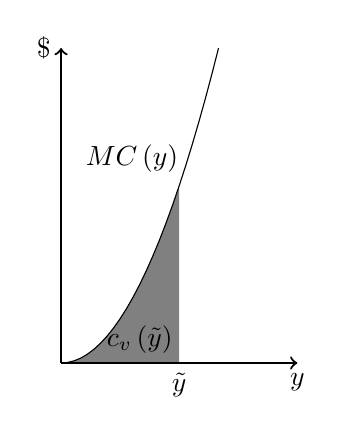
\begin{tikzpicture}
  %\draw[very thin, gray!30, step=1 cm](0,0) grid (4.9,3.9);
    \fill [gray, domain=0:1.5, variable=\x]
    (0, 0)
    -- plot ({\x}, {\x*\x})
    -- (1.5, 0)
    -- cycle;
    \draw [thick] [->] (0,0)--(3,0) node[right, below] {$y$};
    \draw [thick] [->] (0,0)--(0,4) node[above, left] {$\$$};
    \draw [domain=0:2, variable=\x]
    plot ({\x}, {\x*\x}) node at (0.9,2.6) {$MC\left( y \right)$};
    \draw (1, 0.3) node {$c_v\left( \tilde{y} \right)$};
    \draw (1.5, 0) node[below] {$\tilde{y}$};
  \end{tikzpicture}
\end{center}


\section{Firm Supply}
\begin{itemize}
  \item A market is \emph{purely competitive} if the output of each individual
    firm is independent of the market price. Each firm is a \emph{price taker}.
  \item If a firm charges higher than the market price, the firm will have zero
    demand for its output. If the firm charges lower than the market price, it
    will get the entire market demanding its output.
\end{itemize}
An individual firm's demand curve:
\begin{center}
  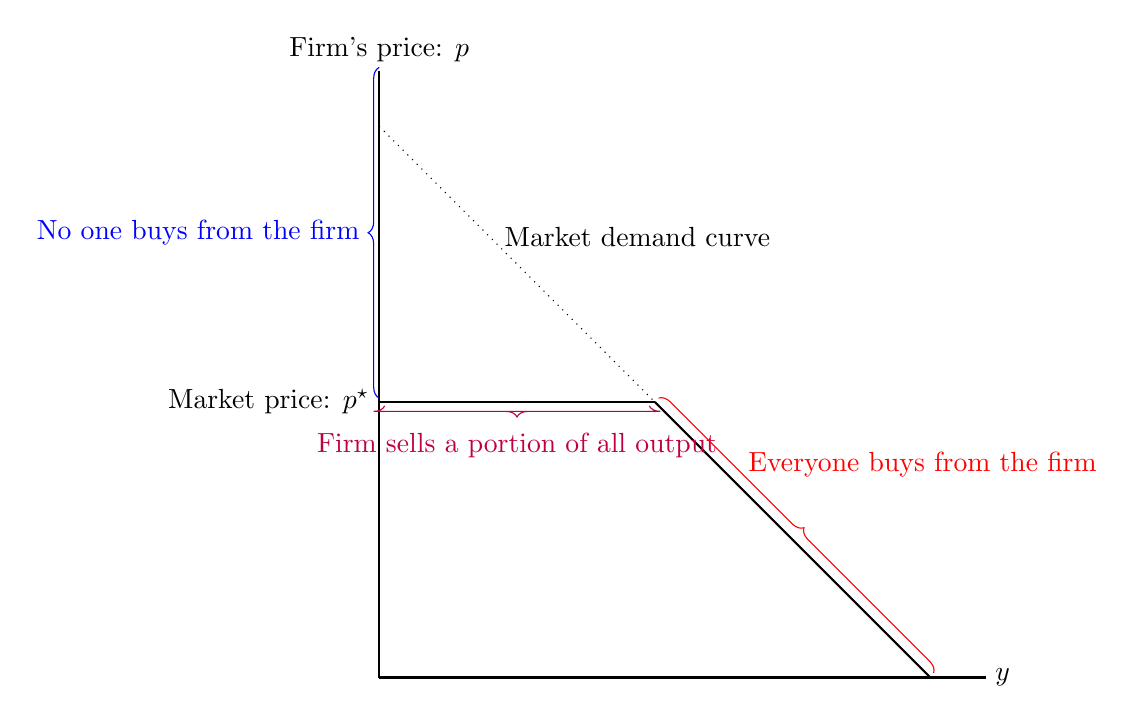
\begin{tikzpicture}[scale=0.7]
    \draw [thick] (0,0) -- (11,0);
    \draw [thick] (0,0) -- (0,11);
    \node [right] at (11,0) {$y$};
    \node [above] at (0,11) {Firm's price: $p$};
    \draw [thick] (0,5) -- (5,5);
    \draw [dotted] (0,10) -- (5,5);
    \draw [thick] (5,5) -- (10,0);
    \node [right] at (2.1,8) {Market demand curve};
    \node [left] at (0,5) {Market price: $p^\star$};
    \draw [blue,decorate,decoration={brace,amplitude=4pt},xshift=0pt,yshift=2pt]
    (0,5) -- (0,11) node [midway,xshift=-2.3cm] {No one buys from the firm};
    \draw [purple,decorate,decoration={brace,amplitude=-4pt},xshift=0pt,yshift=-2pt]
    (0.1,5) -- (4.9,5) node [midway,yshift=-0.5cm] {Firm sells a portion of all output};
    \draw [red,decorate,decoration={brace,amplitude=4pt},xshift=2pt,yshift=2pt]
    (5,5) -- (10,0) node [midway,yshift=0.9cm,xshift=1.6cm] {Everyone buys from the firm};
  \end{tikzpicture}
\end{center}

\begin{itemize}
  \item The firm's maximization problem is:
    \[
    \underset{y}{\max}\; \underbrace{py}_{\text{Revenue}} - \underbrace{
    c\left( y \right)}_{\text{Costs}}\;\;\;\; \text{ where }y\geq 0
    \]
  \item Taking the derivative and setting it equal to zero:
    \[
      p - c^\prime\left( y^\star \right) = 0 \;\;\;\;\Longleftrightarrow\;\;\;\;
      p = c^\prime\left( y^\star \right) \;\;\;\;\Longleftrightarrow\;\;\;\;
      \underbrace{p}_{\text{Marginal revenue}} = \underbrace{MC\left( y^\star
      \right)}_{\text{Marginal cost}}
    \]
  \item For example, if $c\left( y \right)=y^2+1$, the marginal cost is $MC\left( y \right)=2y$. The optimal choice is to set $p=MC\left( y \right)$ so $p=2y$ or $y=\frac{p}{2}$.
  \item The profits from producing nothing is $-F$. Your loss equals the fixed cost.
  \item If the profits from producing nothing is higher (less negative) than the profits from producing where $p=MC\left( y^\star \right)$, then the firm should temporarily shut down.
  \item The firm should shut down when:
    \begin{align*}
      -F &> py^\star - c_v\left( y^\star \right)-F \\
      c_v\left( y^\star \right) &> py^\star  \\
      \frac{c_v\left( y^\star \right)}{y^\star} &> p \\
      AVC\left( y^\star \right) &> p
    \end{align*}
  \item The supply curve of the firm, $S\left( p \right)$ gives the amount of
    output the firm will produce given price. In the short run, this is:
    \[
      S\left( p \right)=
      \begin{cases}
        y^\star \text{ where } p=MC\left( y^\star \right) & \text{ if } p\geq
        AVC\left( y^\star \right) \\
        0 & \text{ if } p<
        AVC\left( y^\star \right) \\
      \end{cases}
    \]
\end{itemize}
\begin{itemize}
  \item The supply curve of the firm is the marginal cost curve when the price exceeds the minimum of average variable cost (solid line) and is zero otherwise:
\end{itemize}
\begin{center}
  \begin{tikzpicture}[scale=0.7]
    \begin{axis}[ticks=none,
                 xmax=10,xmin=-2,
                 ymin=-15,ymax=100,
                 axis lines=middle,
                 width=13cm,
               xlabel=$y$,ylabel=\hspace{-8mm}$\$$]
      \addplot[dashed, samples=100][domain=0:10] {15/x + 50-8*x+x^2};
      \addplot[dashed, black, samples=100][domain=0:10] {50-8*x+x^2};
      \addplot[dotted, black, samples=100][domain=0:10] {50-16*x+3*x^2};
      \addplot[thick, black, samples=100][domain=4:10] {50-16*x+3*x^2};
      \draw (8, 60) node {$AC$};
      \draw (9, 50) node {$AVC$};
      \draw (7.5, 80) node {$MC$};
      \draw [dotted] (0,33.67) -- (4,33.67);
      \draw [black,decorate,decoration={brace,amplitude=4pt},xshift=0pt,yshift=0pt]
      (0,0) -- (0,33.67) node [midway,xshift=-1.1cm] {Shut down};
    \end{axis}
  \end{tikzpicture}
\end{center}
\begin{itemize}
  \item Firm profits can be written as $py^\star - c\left( y^\star
    \right)=py^\star - \frac{c\left( y^\star \right)}{y^\star}y^\star =
    py^\star - AC\left( y^\star \right)y^\star = \left[ p-AC\left( y^\star
    \right) \right]y^\star$.
  \item Graphically, this is the area between the price and the average cost curve, up to the amount produced:
\end{itemize}

\begin{center}
  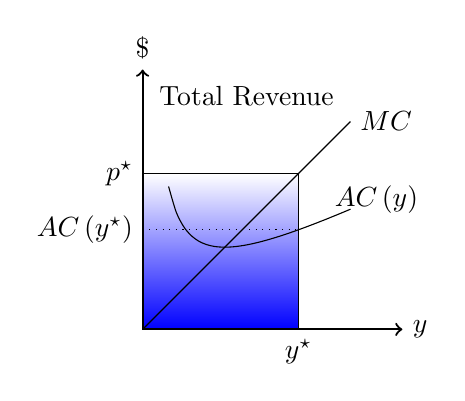
\begin{tikzpicture}[scale=0.33]
    \draw (4, 9) node {Total Revenue};
    \draw[top color=white,bottom color=blue] (0,0) -- (6,0) -- (6,6) -- (0,6);
    \draw[thick,<->] (0,10) node[above] {$\$$}--(0,0)--(10,0) node[right] {$y$};
    \draw (0,0) -- (8, 8) node[right] {$MC$};
    \draw[dotted] (0,6) node[left] {$p^\star$} -- (6, 6) ;
    \draw[dotted] (0,3.83) node[left] {$AC\left( y^\star \right)$} -- (6, 3.83) ;
    \draw[dotted] (6,6)  -- (6, 0) node[below] {$y^\star$};
    \draw[scale=1,domain=1:8,smooth,variable=\x] plot ({\x},{5/\x+0.5*\x});
    \draw (9,5) node {$AC\left( y \right)$};
  \end{tikzpicture}
  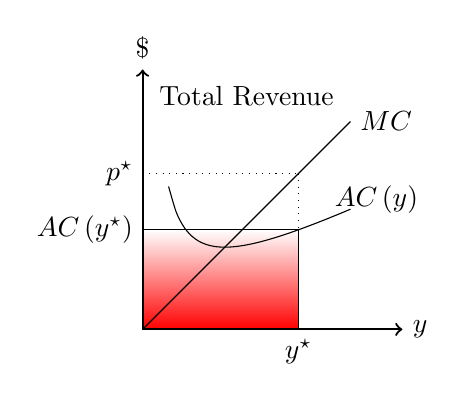
\begin{tikzpicture}[scale=0.33]
    \draw (4, 9) node {Total Revenue};
    \draw[top color=white,bottom color=red] (0,0) -- (6,0) -- (6,3.83) -- (0,3.83);
    \draw[thick,<->] (0,10) node[above] {$\$$}--(0,0)--(10,0) node[right] {$y$};
    \draw (0,0) -- (8, 8) node[right] {$MC$};
    \draw[dotted] (0,6) node[left] {$p^\star$} -- (6, 6) ;
    \draw[dotted] (0,3.83) node[left] {$AC\left( y^\star \right)$} -- (6, 3.83) ;
    \draw[dotted] (6,6)  -- (6, 0) node[below] {$y^\star$};
    \draw[scale=1,domain=1:8,smooth,variable=\x] plot ({\x},{5/\x+0.5*\x});
    \draw (9,5) node {$AC\left( y \right)$};
  \end{tikzpicture}
  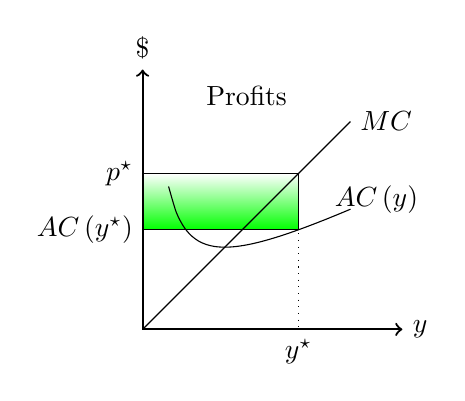
\begin{tikzpicture}[scale=0.33]
    \draw (4, 9) node {Profits};
    \draw[top color=white,bottom color=green] (0,3.83) -- (6,3.83) -- (6,6) -- (0,6);
    \draw[thick,<->] (0,10) node[above] {$\$$}--(0,0)--(10,0) node[right] {$y$};
    \draw (0,0) -- (8, 8) node[right] {$MC$};
    \draw[dotted] (0,6) node[left] {$p^\star$} -- (6, 6) ;
    \draw[dotted] (0,3.83) node[left] {$AC\left( y^\star \right)$} -- (6, 3.83) ;
    \draw[dotted] (6,6)  -- (6, 0) node[below] {$y^\star$};
    \draw[scale=1,domain=1:8,smooth,variable=\x] plot ({\x},{5/\x+0.5*\x});
    \draw (9,5) node {$AC\left( y \right)$};
  \end{tikzpicture}
\end{center}
\begin{itemize}
  \item \emph{Producer surplus} equals revenues minus variable costs,
    $PS=py-c_v\left( y \right)$.
  \item Producer surplus can be written as:
    \[PS=py-c_v\left( y \right)=py-AVC\left( y \right)\times y = \left[ p-AVC\left( y \right) \right]y\]
  \item Graphically, this is the area between the price and the average variable cost curve:
\end{itemize}
\begin{center}
  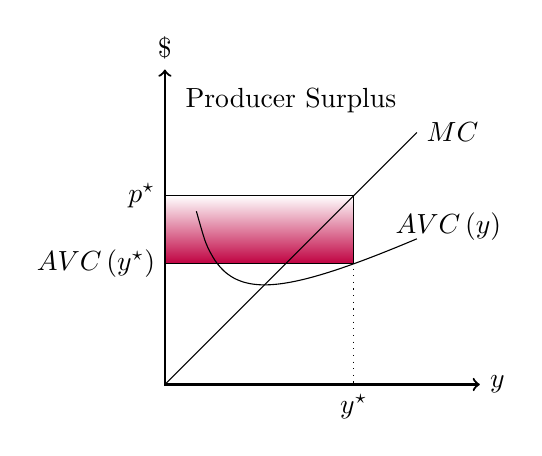
\begin{tikzpicture}[scale=0.4]
    \draw (4, 9) node {Producer Surplus};
    \draw[top color=white,bottom color=purple] (0,3.83) -- (6,3.83) -- (6,6) -- (0,6);
    \draw[thick,<->] (0,10) node[above] {$\$$}--(0,0)--(10,0) node[right] {$y$};
    \draw (0,0) -- (8, 8) node[right] {$MC$};
    \draw[dotted] (0,6) node[left] {$p^\star$} -- (6, 6) ;
    \draw[dotted] (0,3.83) node[left] {$AVC\left( y^\star \right)$} -- (6, 3.83) ;
    \draw[dotted] (6,6)  -- (6, 0) node[below] {$y^\star$};
    \draw[scale=1,domain=1:8,smooth,variable=\x] plot ({\x},{5/\x+0.5*\x});
    \draw (9,5) node {$AVC\left( y \right)$};
  \end{tikzpicture}
\end{center}
\begin{itemize}
  \item The firm will only produce in the long run if profits are nonnegative:
    $py-c\left( y \right)\geq 0$. This happens when price exceeds average cost:
    \[
      py-c\left( y \right)\geq 0 \;\;\;\; \Longleftrightarrow \;\;\;\;
      py \geq c\left( y \right) \;\;\;\; \Longleftrightarrow \;\;\;\;
      p \geq \frac{c\left( y \right)}{y}  \;\;\;\; \Longleftrightarrow \;\;\;\;
      p \geq AC\left( y \right)
    \]
\end{itemize}

\section{Industry Supply}
\begin{itemize}
  \item $S_i\left( p \right)$ is the short-run supply curve for firm $i$. The
    short-run \emph{industry supply curve} when there are are $n$ firms is:
    \[
      S\left( p \right)=S_1\left( p \right)+S_2\left( p \right) + \dots+
      S_n\left( p \right) = \sum_{i=1}^n S_i\left( p \right)
    \]
  \item The intersection of the industry supply curve and the market demand curve
    gives the equilibrium market price $p^\star$.
  \item In the short run, firms set $y^\star$ such that $p^\star = MC\left(
    y^\star \right)$. In the short run, firms could either break even, make
    profits or suffer losses.
\end{itemize}
\begin{center}
  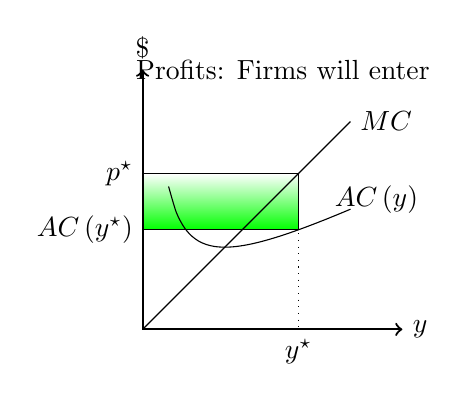
\begin{tikzpicture}[scale=0.33]
    \draw (5.4, 10) node {Profits: Firms will enter};
    \draw[top color=white,bottom color=green] (0,3.83) -- (6,3.83) -- (6,6) -- (0,6);
    \draw[thick,<->] (0,10) node[above] {$\$$}--(0,0)--(10,0) node[right] {$y$};
    \draw (0,0) -- (8, 8) node[right] {$MC$};
    \draw[dotted] (0,6) node[left] {$p^\star$} -- (6, 6) ;
    \draw[dotted] (0,3.83) node[left] {$AC\left( y^\star \right)$} -- (6, 3.83) ;
    \draw[dotted] (6,6)  -- (6, 0) node[below] {$y^\star$};
    \draw[scale=1,domain=1:8,smooth,variable=\x] plot ({\x},{5/\x+0.5*\x});
    \draw (9,5) node {$AC\left( y \right)$};
  \end{tikzpicture}
  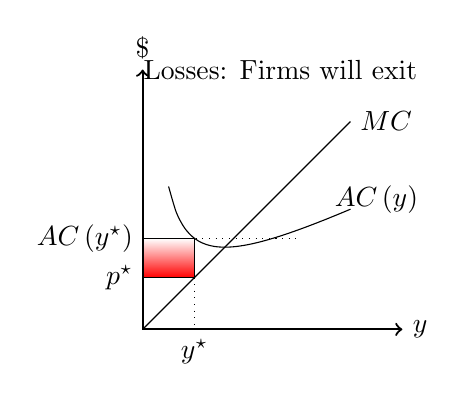
\begin{tikzpicture}[scale=0.33]
    \draw (5.3, 10) node {Losses: Firms will exit};
    \draw[top color=white,bottom color=red] (0,3.5) -- (2,3.5) -- (2,2) -- (0,2);
    \draw[thick,<->] (0,10) node[above] {$\$$}--(0,0)--(10,0) node[right] {$y$};
    \draw (0,0) -- (8, 8) node[right] {$MC$};
    \draw[dotted] (0,2) node[left] {$p^\star$} -- (2, 2) ;
    \draw[dotted] (0,3.5) node[left] {$AC\left( y^\star \right)$} -- (6, 3.5) ;
    \draw[dotted] (2,2)  -- (2, 0) node[below] {$y^\star$};
    \draw[scale=1,domain=1:8,smooth,variable=\x] plot ({\x},{5/\x+0.5*\x});
    \draw (9,5) node {$AC\left( y \right)$};
  \end{tikzpicture}
  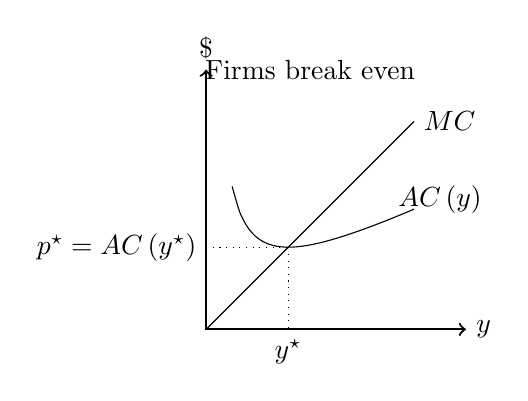
\begin{tikzpicture}[scale=0.33]
    \draw (4, 10) node {Firms break even};
    \draw[thick,<->] (0,10) node[above] {$\$$}--(0,0)--(10,0) node[right] {$y$};
    \draw (0,0) -- (8, 8) node[right] {$MC$};
    \draw[dotted] (0,3.16) node[left] {$p^\star=AC\left( y^\star \right)$} -- (3.16, 3.16) ;
    \draw[dotted] (3.16,3.16)  -- (3.16, 0) node[below] {$y^\star$};
    \draw[scale=1,domain=1:8,smooth,variable=\x] plot ({\x},{5/\x+0.5*\x});
    \draw (9,5) node {$AC\left( y \right)$};
  \end{tikzpicture}
\end{center}
\begin{itemize}
  \item In the long run, if firms are making losses firms will exit until firms
    break even. If firms are making profits, other firms will enter until firms
    break even. This happens when $p^\star = \frac{c\left( y^\star
    \right)}{y^\star}$, where $\frac{c\left( y^\star
    \right)}{y^\star}$ is the minimum average cost.
  \item When firms enter ($n$ increases), the industry supply curve moves to the right. When firms exit ($n$ decreases), the industry supply curve moves to the left. In the long run the industry supply curve will intersect the market demand curve $D\left( p \right)$ at the point where the price equals the minimum of average total cost:
\end{itemize}
\begin{center}
  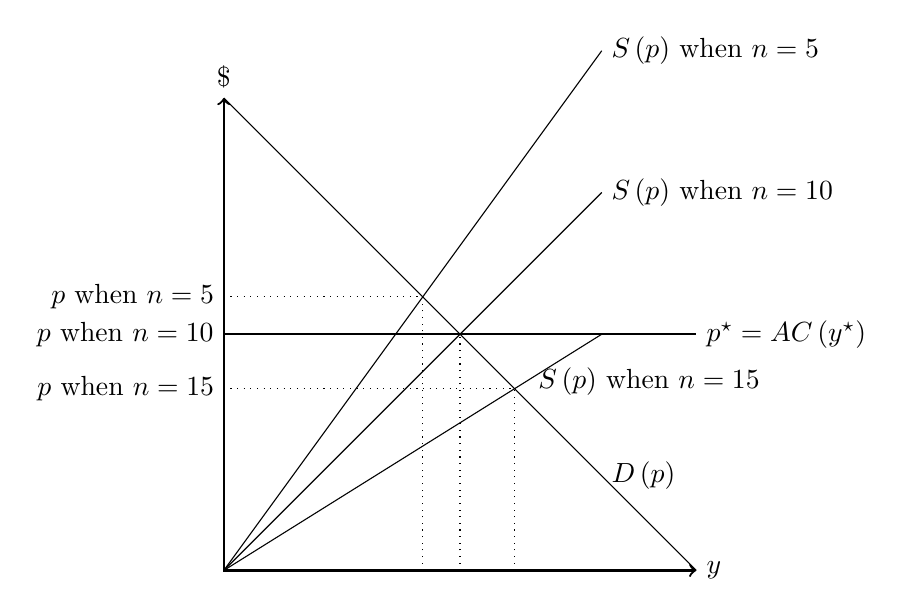
\begin{tikzpicture}[scale=0.6]
    \draw[thick,<->] (0,10) node[above] {$\$$}--(0,0)--(10,0) node[right] {$y$};
    \draw[thick] (0,5) node[left] {$p$ when $n=10$} -- (10, 5) node[right] {$p^\star=AC\left( y^\star \right)$};
    \draw (0,10) -- (10, 0);
    \draw (8, 2) node[right] {$D\left( p \right)$};
    \draw (0,0) -- (8, 8) node[right] {$S\left( p \right)$ when $n=10$};
    \draw (0,0) -- (8, 11) node[right] {$S\left( p \right)$ when $n=5$};
    \draw (0,0) -- (8, 5);
    \draw (9, 4) node {$S\left( p \right)$ when $n=15$};
    \draw[dotted] (0,5.8) node[left] {$p$ when $n=5$} -- (4.2, 5.8) ;
    \draw[dotted] (0,3.85) node[left] {$p$ when $n=15$} -- (6.15, 3.85) ;
    \draw[dotted] (4.2,0)  -- (4.2, 5.8) ;
    \draw[dotted] (5,0) -- (5, 5) ;
    \draw[dotted] (6.15,0) -- (6.15, 3.85) ;
  \end{tikzpicture}
\end{center}

\section{Equilibrium}
\begin{itemize}
  \item The equilibrium price of a good, $p^\star$, is the price where the
    market supply of the good equals market demand. It is the $p^\star$ that
    solves $D\left( p^\star \right)=S\left( p^\star \right)$.
\end{itemize}
\emph{Example}\par\noindent
Suppose we have a demand curve $D\left( p \right)=a-bp$ and supply curve $S\left( p \right)=c+dp$. To find the equilibrium price $p^\star$, we set $D\left( p^\star \right)=S\left( p^\star \right)$:
\begin{align*}
  a-bp^\star &= c +dp^\star \\
  a-c&= bp^\star  +dp^\star \\
  a-c&= p^\star \left( b+d \right) \\
  p^\star &= \frac{a-c}{b+d} \\
\end{align*}
To find the equilibrium quantity, use $p^\star$ in either the demand or supply curve. Suppose we used the demand curve:
\begin{align*}
  q^\star = a - bp^\star = a - b\left(\frac{a-c}{b+d}  \right) = \frac{a\left( b+d \right)-b\left( a-c \right)}{b+d} =\frac{ab + ad -ab +bc}{b+d}=\frac{ad+bc}{b+d}
\end{align*}
\begin{itemize}
  \item The inverse demand curve, $P_D\left( q \right)$, is the price
    demanders are willing to pay to consume a particular quantity.
  \item The inverse supply curve, $P_S\left( q \right)$, is the price suppliers
    must receive in order to supply a particular quantity.
\end{itemize}
\emph{Example}\par\noindent
To find the inverse demand curve of the above example $D\left( p \right)=a-bp$, we simply solve for $p$:
\begin{align*}
  q&=a-bp  \\
 bp &=a-q  \\
 p &=\frac{a}{b}-\frac{1}{b}q  \\
 P_D\left( q \right) &=\frac{a}{b}-\frac{1}{b}q  \\
\end{align*}
We can do the same for supply to find $P_S\left( q \right)=\frac{q}{d}-\frac{c}{d}$.
\begin{itemize}
  \item In equilibrium, $P_S\left( q^\star \right)=P_D\left( q^\star \right)$,
    where $q^\star$ is the quantity produced in equilibrium.
  \item Factors other than price that change demand or supply cause shifts in the demand and supply curves. When price changes we simply move along the curve.
  \item Changes in technology and input prices are some of the things that cause the supply curve to shift.
  \item Changes in preferences, prices of other goods and income are some the things that cause the demand curve to shift.
\end{itemize}
Comparative statics of demand and supply shifts:
\begin{center}
  \begin{tabular}{|l|l|}\hline
    If $S\uparrow$ (outward shift)& $p\downarrow$ and $q\uparrow$ \\\hline
    If $S\downarrow$ (inward shift)& $p\uparrow$ and $q\downarrow$ \\\hline
    If $D\uparrow$ (outward shift)& $p\uparrow$ and $q\uparrow$ \\\hline
    If $D\downarrow$ (inward shift) & $p\downarrow$ and $q\downarrow$ \\\hline
  \end{tabular}
\end{center}
\subsubsection*{Quantity Taxes}
\begin{itemize}
  \item A \emph{quantity tax} is a tax levied per unit of quantity bought or sold. For example, there might be a quantity tax of \$3 on each packet of cigarettes.
  \item If there is a quantity tax $t$, then $P_D=P_S+t$, where $P_D$ is the price consumers pay and $P_S$ is the price sellers receive. The difference in the price consumers pay and the price suppliers receive is the quantity tax.
\end{itemize}
\emph{Example}\par\noindent
Suppose again that $D\left( P_D \right)=a-bP_D$ and $S\left( P_S \right)=c+dP_S$. With a quantity tax, $P_D=P_S+t$. Substituting into the demand function give: $D\left( P_S \right)=a-b\left(P_S+t  \right)=a-bP_S-bt$. In equilibrium we will have:
\begin{align*}
  a-bP_S-bt&=c+dP_S\\
  -dP_S -bP_S&=bt + c-a\\
  dP_S+ bP_S&=a - c - bt\\
  P_S \left( b+d \right)&=a - c - bt\\
  P_S &=\frac{a-c-bt}{b+d}\\
\end{align*}
Before the tax we had $p=\frac{a-c}{b+d}$ so $P_S$ is lower now by $\frac{bt}{b+d}$. Sellers receive less for each unit sold. We can also calculate $P_D$:
\begin{equation*}
  P_D=P_S+t = \frac{a-c-bt}{b+d} + t = \frac{a-c-bt +t\left( b+d \right)}{b+d}=
  \frac{a-c-bt+bt+dt}{b+d}=\frac{a-c+dt}{b+d}
\end{equation*}
$P_D$ is therefore higher by $\frac{dt}{b+d}$. Consumers pay more for each unit with the tax.
\subsubsection*{Value Taxes}
\begin{itemize}
  \item A \emph{value tax} is a tax expressed in percentage units. The sales tax that we see is an example of a value tax. If the price is \$1 and the value tax is 5\%, then the final price is \$1.05.
  \item If there is a value tax $\tau$, then $P_D=\left( 1+\tau \right)P_S$.
\end{itemize}
\subsubsection*{Tax Incidence}
\begin{center}
\begin{tikzpicture}[domain=0:5,scale=1,thick]
\usetikzlibrary{calc}                                %allows coordinate calculations.
\usetikzlibrary{decorations.pathreplacing}           %allows drawing curly braces.
\def\dint{4.5}      %Y-intercept for DEMAND.
\def\dslp{-0.5}     %Slope for DEMAND.
\def\sint{1.2}      %Y-intercept for SUPPLY.
\def\sslp{0.8}      %Slope for SUPPLY.
\def\tax{1.5}       %Excise (per-unit) tax
% Define Supply and Demand Lines as equations of parameters defined above.
  \def\demand{\x,{\dslp*\x+\dint}}
  \def\supply{\x,{\sslp*\x+\sint}}
  \def\demandtwo{\x,{\dslp*\x+\dint+\dsh}}
  \def\supplytwo{\x,{\sslp*\x+\sint+\ssh}}
% Define coordinates.
    \coordinate (ints) at ({(\sint-\dint)/(\dslp-\sslp)},{(\sint-\dint)/(\dslp-\sslp)*\sslp+\sint});
    \coordinate (ep) at  (0,{(\sint-\dint)/(\dslp-\sslp)*\sslp+\sint});
    \coordinate (eq) at  ({(\sint-\dint)/(\dslp-\sslp)},0);
    \coordinate (dint) at (0,{\dint});
    \coordinate (sint) at (0,{\sint});
    \coordinate (teq) at  ({(\sint+\tax-\dint)/(\dslp-\sslp)},0); %quantity
    \coordinate (tep) at  (0,{(\sint+\tax-\dint)/(\dslp-\sslp)*\sslp+\sint+\tax}); %price
    \coordinate (tint) at  ({(\sint+\tax-\dint)/(\dslp-\sslp)},{(\sint+\tax-\dint)/(\dslp-\sslp)*\sslp+\sint+\tax}); %tax equilibrium

    \coordinate (sep) at (0,{\sslp*(\sint+\tax-\dint)/(\dslp-\sslp)+\sint});
    \coordinate (sen) at ({(\sint+\tax-\dint)/(\dslp-\sslp)},{\sslp*(\sint+\tax-\dint)/(\dslp-\sslp)+\sint});

% DEMAND
    \draw[thick,color=blue] plot (\demand) node[right] {Demand};
% SUPPLY
    \draw[thick,color=purple] plot (\supply) node[right] {Supply};
% Draw axes, and dotted equilibrium lines.
    \draw[->] (0,0) -- (6.2,0) node[right] {$q$};
    \draw[->] (0,0) -- (0,6.2) node[above] {$p$};
    \draw[decorate,decoration={brace},thick]  ($(sep)+(-0.8,0)$) -- ($(tep)+(-0.8,0)$) node[midway,below=-8pt,xshift=-18pt] {tax};
    \draw[dashed] (tint) -- (teq) node[below] {$q_T$};
    \draw[dashed] (tint) -- (tep) node[left] {$P_d$};
    \draw[dashed] (sen) -- (sep) node[left] {$P_s$};
\end{tikzpicture}
\end{center}
\begin{itemize}
  \item If the pre-tax equilibrium price was $p^\star$, then the portion of the
    tax that consumers pay is:
    \[
      \frac{P_D-p^\star}{t}
    \]
    The portion of the tax that sellers pay is:
    \[
      \frac{p^\star - P_S}{t}
    \]
\end{itemize}
\emph{Example}\par\noindent
In the example above with the quantity tax, the portion of the tax that consumers paid is:
\begin{equation*}
  \frac{P_D-p^\star}{t} =\frac{ \frac{a-c+dt}{b+d}-\frac{a-c}{b+d}}{t}=\frac{\frac{dt}{b+d}}{t} = \frac{d}{b+d}
\end{equation*}
The portion that sellers paid is:
\begin{equation*}
  \frac{p^\star-P_S}{t} = \frac{\frac{a-c}{b+d}-\frac{a-c-bt}{b+d}}{t}=\frac{\frac{bt}{b+d}}{t}=\frac{b}{b+d}
\end{equation*}
The portions of the tax depend on the slopes of the demand and supply curves. The steeper the slope, the larger portion of the tax you pay.
\begin{itemize}
  \item The burden of the tax falls on the relatively less elastic side (buyers or sellers).
  \item If demand is perfectly inelastic, consumers pay all of the tax.
  \item If supply is perfectly inelastic, suppliers pay all of the tax.
  \item If demand is perfectly elastic, suppliers pay all of the tax.
  \item If supply is perfectly elastic, consumers pay all of the tax.
\end{itemize}
\subsubsection*{Pareto Efficiency}
\begin{itemize}
  \item An economic situation is \emph{Pareto efficient} if there is no way to make
    any person better off without hurting anyone else.
  \item The market equilibrium without taxes is Pareto efficient.
  \item In the left diagram below, there is no tax. Consumer surplus is shown in blue and producer surplus is shown in red.
  \item In the right diagram below, there is a tax. The consumer surplus is the smaller blue triangle. The producer surplus is the smaller red triangle. The green rectangle is government revenue which is the tax per unit multiplied by the number of units sold $t \times q_T$. The remaining area (in gray) is the deadweight loss.
\end{itemize}
\begin{center}
  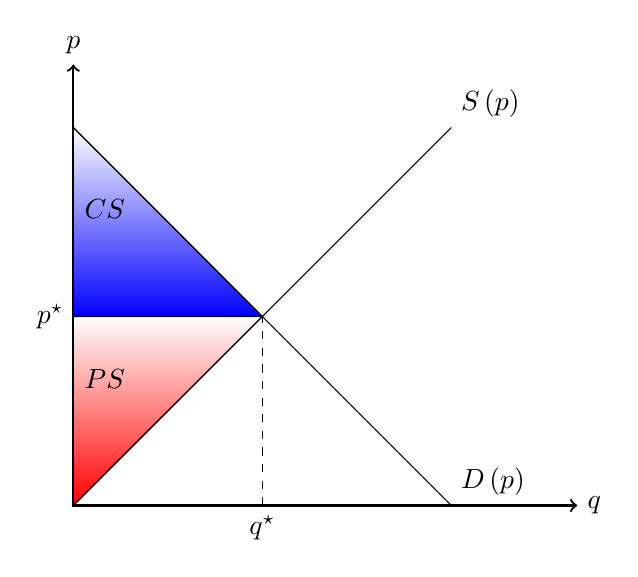
\begin{tikzpicture}[scale=0.8]
    \draw[thick,<->] (0,7) node[above] {$p$}--(0,0)--(8,0) node[right] {$q$};
    \draw[top color=white,bottom color=blue] (0,6) -- (0,3) -- (3,3) -- cycle;
    \draw (0.5,4.7) node[black] {$CS$};
    \draw[top color=white,bottom color=red] (0,0) -- (0,3) -- (3,3) -- cycle;
    \draw (0.5,2) node[black] {$PS$};
    \draw[dashed,-] (3,0) node[below] {$q^\star$} -- (3,3);
    \draw[dashed,-] (0,3) node[left] {$p^\star$} -- (3,3);
    \draw (0,6)--(6,0);
    \draw (0,0)--(6,6) node[above right] {$S\left( p \right)$};
    \draw (6,0) node[above right] {$D\left( p \right)$};
  \end{tikzpicture}
  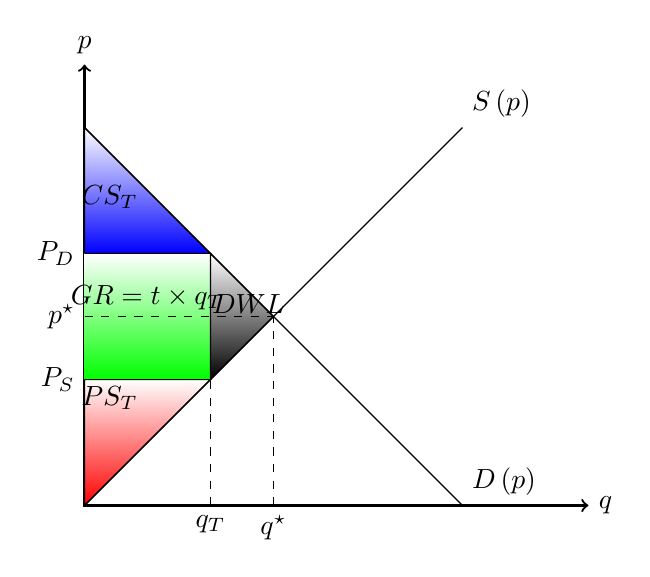
\begin{tikzpicture}[scale=0.8]
    \draw[thick,<->] (0,7) node[above] {$p$}--(0,0)--(8,0) node[right] {$q$};
    \draw[top color=white,bottom color=blue] (0,4) -- (2,4) -- (0,6) -- cycle;
    \draw[top color=white,bottom color=red] (0,0) -- (2,2) -- (0,2) -- cycle;
    \draw[top color=white,bottom color=green] (0,2) -- (2,2) -- (2,4) -- (0,4);
    \draw[top color=white,bottom color=black] (2,2) -- (2,4) -- (3,3) -- cycle;
    \draw (0.4,4.9) node[black] {$CS_T$};
    \draw (0.4,1.7) node[black] {$PS_T$};
    \draw (1,3.3) node[black] {$GR=t\times q_T$};
    \draw (2.6,3.2) node[black] {$DWL$};
    \draw[dashed,-] (3,0) node[below] {$q^\star$} -- (3,3);
    \draw[dashed,-] (2,0) node[below] {$q_T$} -- (2,2);
    \draw[dashed,-] (0,2) node[left] {$P_S$} -- (2,2);
    \draw[dashed,-] (0,4) node[left] {$P_D$} -- (2,4);
    \draw[dashed,-] (0,3) node[left] {$p^\star$} -- (3,3);
    \draw (0,6)--(6,0);
    \draw (0,0)--(6,6) node[above right] {$S\left( p \right)$};
    \draw (6,0) node[above right] {$D\left( p \right)$};
  \end{tikzpicture}
\end{center}
\section{Demand Elasticities}
Elasticity measures the responsiveness of demand. The slope of the demand curve is a potentially a good measure of responsiveness, but it depends on the units. For example, suppose you were interested in the demand for gasoline. If you change the units from gallons to liters, the elasticity would change. We should have a unit-free measure. Therefore we define the own-price elasticity of demand as:
\[
  \varepsilon = \frac{\nicefrac{\Delta q}{q}}{\nicefrac{\Delta p }{p}}
\]
If the change in price is small, we can use the derivative of demand with respect to price:
\[
  \varepsilon = \frac{dq}{dp}\frac{p}{q}
\]
If we are using an individual's demand function for good 1 $x_1\left( p_1,p_2,m \right)$, this is:
\[
  \varepsilon = \frac{dx_1\left( p_1,p_2,m \right)}{dp_1}\frac{p_1}{x_1}
\]
For most goods (non-Giffen goods), the elasticity of demand with respect to price will be negative. Therefore we will often talk about the elasticity in terms of absolute value, $\left| \varepsilon \right|$.

If $\left| \varepsilon \right|>1$, demand is \emph{elastic}. If $\left| \varepsilon \right|<1$, demand is \emph{inelastic}. If $\left| \varepsilon \right|=1$, demand is \emph{unit elastic}.

Elasticity can be higher or lower depending on the substitutability of a good. A good with many substitutes will be more elastic than one with fewer.
\subsubsection*{Elasticity and Revenue}
Revenue is equal to price times quantity: $R=pq$. If the price changes from $p$ to $p+\Delta p$, then the quantity demanded will change from $q$ to $q+\Delta q$. Revenue will then be:
\[
  R+\Delta R= \left( p+\Delta p \right)\left( q + \Delta q \right)=\underbrace{pq}_{=R} + \Delta p q + p\Delta q + \underbrace{\Delta p \Delta q}_{\approx 0 \text{ if } \Delta p \text{ small}}
\]
The change in revenue is therefore approximately:
\[
  \Delta R = \Delta p q + p\Delta q
\]
  \begin{tikzpicture}[scale=1]
    \draw [thick] (0,0) -- (7,0);
    \draw [thick] (0,0) -- (0,7);
    \node [right] at (7,0) {$q$};
    \node [above] at (0,7) {$p$};
    \draw [thick] (0,6) -- (6,0);
    \node [left] at (0,3) {$p+\Delta p$};
    \draw[dotted](0,3)--(4,3);
    \node [left] at (0,2) {$p$};
    \draw[dotted](0,2)--(4,2);
    \node [below] at (3,0) {$q+\Delta q$};
    \draw[dotted](3,0)--(3,3);
    \node [below] at (4,0) {$q$};
    \draw[dotted](4,0)--(4,3);
    \node[blue] at (1.5, 2.5) {\Large{$A$}};
    \node[blue] at (3.5, 2.5) {\Large{$B$}};
    \node[blue] at (1.5, 1.0) {\Large{$C$}};
    \node[blue] at (3.5, 1.0) {\Large{$D$}};
  \end{tikzpicture}

  At $p$ and $q$, the revenue in the diagram is $C+D$. At the new price and quantity $p+\Delta p$ and $q+\Delta q$, the revenue is $A+C$. The change in revenue is therefore $A-D$ Here, $p\Delta q$ is the negative of box $D$ and $\Delta p q$ is $A+B$, but $B\approx 0$ for small changes in price. So the change in revenue, $\Delta R = \Delta p q + p \Delta q$, is the box $A$ minus the box $D$.

If we divide the change in revenue formula by $\Delta p$:
\[
  \frac{\Delta R}{\Delta p} = \frac{\Delta p q}{\Delta p} + p\frac{\Delta q}{\Delta p} = q + p\frac{\Delta q}{\Delta p}\frac{p}{p}=q\left( 1+\frac{\Delta q}{\Delta p}\frac{p}{q} \right)=q\left( 1+ \varepsilon\right)=q\left( 1-\left| \varepsilon \right| \right)
\]
If $\left| \varepsilon \right|>1$, then revenue decreases when price increases. If $\left| \varepsilon \right|<1$, then revenue increases when price increases. If $\left| \varepsilon \right|=1$, then revenue doesn't change when price increases.
\subsubsection*{Marginal Revenue}
Marginal revenue is the change in revenue from producing a small increase in quantity. For price-takers (in perfect competition), this was always just the price, as their output didn't affect the market price. More generally, however, if a firm produces more output, this can affect the price of output. Dividing the change in revenue formula by the change in quantity:
\[
  \frac{\Delta R}{\Delta q} = \frac{p\Delta q}{\Delta q} + q\frac{\Delta p}{\Delta q}=p+q\frac{\Delta p}{\Delta q}\frac{p}{p}=p+\frac{q}{p}\frac{\Delta p}{\Delta q}p = p + \frac{1}{\varepsilon}p=p\left( 1+\frac{1}{\varepsilon} \right)=p\left( 1-\frac{1}{\left| \varepsilon \right|} \right)
\]
If demand is elastic, $\left| \varepsilon \right|>1$, then revenue increases when quantity increases. If demand is inelastic, $\left| \varepsilon \right|<1$, then revenue decreases when quantity increases. If demand is unit elastic, $\left| \varepsilon \right|=1$, then revenue doesn't change when quantity increases.

To see the above with derivatives instead of small changes, we can use the product rule on the revenue function expressed in quantities: $R\left( q \right)=p\left( q \right)\times q$:
\[
  \frac{dR\left( q \right)}{dq}= p\left( q \right)\times 1 +\frac{dp}{dq}q =
  p + \frac{dp}{dq}\frac{qp}{p}= p\left( 1+ \frac{dp}{dq}\frac{q}{p}\right)=
  p\left( 1+\frac{1}{\varepsilon} \right)=p\left( 1-\frac{1}{\left| \varepsilon \right|} \right)
\]
\subsubsection*{Example with linear demand}
\begin{multicols}{2}
\begin{itemize}
    \item Suppose the inverse demand function is $p\left( q \right)=a - bq$.
    \item The revenue function is $R\left( q \right)=p\left( q \right)\times
      q=\left[ a-bq \right]q = aq - bq^2$.
    \item Marginal revenue is then $MR\left( q \right)=\frac{dR\left( q
      \right)}{dq}=a - 2bq$.
    \item The inverse demand function meets the vertical axis at $a$ and the horizontal axis at $\frac{a}{b}$.
    \item The marginal revenue function also meets the vertical axis at $a$ and the horizontal axis at $\frac{a}{2b}$ --- exactly half way towards the demand curve.
    \item $MR\left( q \right)$ is positive only when $\left| \varepsilon
      \right|>1$.
  \end{itemize}
  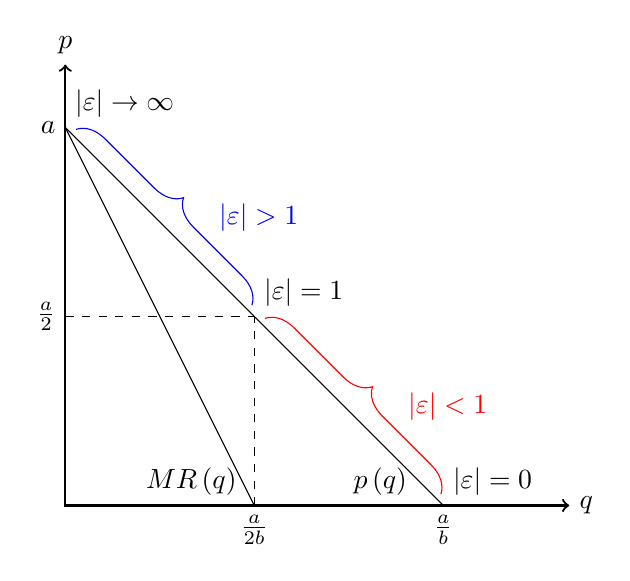
\begin{tikzpicture}[scale=0.8]
    \draw[thick,<->] (0,7) node[above] {$p$}--(0,0)--(8,0) node[right] {$q$};
    \draw (0,6) node[left] {$a$};
    \draw[dashed,-] (0,3) node[left] {$\frac{a}{2}$} (0,3)--(3,3);
    \draw[dashed,-] (3,0) node[below] {$\frac{a}{2b}$} (3,0)--(3,3);
    \draw (6,0) node[below] {$\frac{a}{b}$};
    \draw (0,6)--(6,0);
    \draw (0,6)--(3,0);
    \draw (5,0) node[above] {$p\left( q \right)$};
    \draw (2,0) node[above] {$MR\left( q \right)$};
    \draw[blue,decorate,decoration={brace, amplitude=10pt},xshift=2pt,yshift=2pt]
    (0.1,5.9) -- (2.9,3.1) node [blue,midway,xshift=1.2cm] {$\left| \varepsilon
      \right|>1$};
    \draw[red,decorate,decoration={brace, amplitude=10pt},xshift=2pt,yshift=2pt]
    (3.1,2.9) -- (5.9,0.1) node [red,midway,xshift=1.2cm] {$\left| \varepsilon
      \right|<1$};
    \draw (3,3) node[above right] {$\left| \varepsilon \right|=1$};
    \draw (0,6) node[above right] {$\left| \varepsilon \right|\rightarrow
    \infty$};
    \draw (6,0) node[above right] {$\left| \varepsilon \right|=0$};
  \end{tikzpicture}
\end{multicols}
\subsubsection*{Different Types of Demand Elasticities}
So far we have been talking about the \emph{own-price} elasticity of demand. However, there are other types of elasticities:
\begin{itemize}
  \item The \emph{cross-price elasticity} measures the sensitivity of the demand
    for good 1 when the price of good 2 changes (or vice versa). It is defined
    by $\varepsilon_{12} = \frac{dq_1}{dp_2}\frac{p_2}{q_1}$.
    \begin{itemize}
      \item If $ \varepsilon_{12}>0$, then the goods are
        substitutes. If $\varepsilon_{12}<0$, then the goods are
        complements.
    \end{itemize}
  \item The \emph{income elasticity} measures the sensitivity of demand with
    income: $\eta=\frac{dq}{dm}\frac{m}{q}$.
    \begin{itemize}
      \item If $\eta>0$, the good is normal. If $\eta<0$, the good is inferior.
        If $\eta>1$, the good is a luxury good.
    \end{itemize}
\end{itemize}
Suppose we have a Cobb-Douglas utility function $u\left( x_1,x_2 \right)=x_1^ax_2^b$, where as we have shown before the demand functions are $x_1\left( p_1,p_2,m \right)=\frac{a}{a+b}\frac{m}{p_1}$ and $x_2\left( p_1,p_2,m \right)=\frac{b}{a+b}\frac{m}{p_2}$
The own-price elasticity of demand for good 1 is:
\[
  \varepsilon_1 = \frac{\partial x_1}{\partial p_1}\frac{p_1}{x_1}=\underbrace{\left(-\left( \frac{a}{a+b} \right)\frac{m}{p_1^2}\right)}_{\frac{\partial x_1}{\partial  p_1}}\frac{p_1}{x_1}=\left(-\left( \frac{a}{a+b} \right)\frac{m}{p_1^2}\right)\frac{p_1}{\frac{a}{a+b}\frac{m}{p_1}}=-1
\]
The cross-price elasticity of demand for good 1 with respect to good 2 is zero, as the price of good 2 is not in the demand function for good 1.

The income elasticity of demand for good 1 is:
\[  \eta_1 =
  \frac{\partial x_1}{\partial m}\frac{m}{x_1}=\underbrace{\left( \frac{a}{a+b}\frac{1}{p_1}\right)}_{\frac{\partial x_1}{\partial  m}}\frac{m}{x_1}=
  \left( \frac{a}{a+b}\frac{1}{p_1}\right)\frac{m}{\frac{a}{a+b}\frac{m}{p_1}} = 1
\]
\section{Monopoly}
In monopoly, there is only one firm. Unlike perfect competition, price is no longer given. When the monopolist is choosing the optimal quantity, it knows the effect of the quantity on the price.

The monopolist's problem is: $\underset{q}{\max}\; R\left( q \right)-c\left( q \right)$. The optimality condition is then $R^\prime\left( q \right)=c^\prime\left( q \right)$, or $MR\left( q \right)=MC\left( q \right)$.

The revenue function is $R\left( q \right)=p\left( q \right)\times q$. We could write the monopolist's problem as $\underset{q}{\max}\; p\left( q \right)q-c\left( q \right)$. At the optimal quantity:
\[
  p\left( q \right) + p^\prime\left( q \right)q - c^\prime\left( q \right)=0
\]
So $p\left( q \right)=c^\prime\left( q \right)-p^\prime\left( q \right)q$. In perfect competition, the firms set $p=MC\left( q \right)$. Here, the monopolist sets price equal to marginal cost \emph{plus} a margin over marginal cost, where the margin is $-p^\prime\left( q \right)q$.

From before, we saw that we can write marginal revenue as $p\left( q \right)\left[ 1-\frac{1}{\left| \varepsilon \right|} \right]$. So the monopolist charges a markup over marginal cost of:
\[p\left( q
    \right)=\underbrace{\left(\frac{1}{1-\frac{1}{\left| \varepsilon\left( q
  \right) \right|}}\right)}_{\text{Mark-up}} MC\left( q \right)
\]
From the mark-up we can see that the monoplist will always set a price in the elastic part of the demand curve ($\left| \varepsilon\left( q \right) \right|>1$).
\subsubsection*{Example with linear inverse demand}
The inverse demand function is $p\left( q \right)=a-bq$ and the cost function is $cq$. Marginal cost is therefore $c$. The profit for the monopolist is:
\[
  \pi\left( q \right)=p\left(q \right)q - c\left( q \right) = \left( a-bq \right)q-cq=aq - bq^2 - cq
\]
Maximizing this function:
\[
  a-2bq-c=0 \;\;\;\Longrightarrow\;\;\;
  2bq=a-c \;\;\;\Longrightarrow\;\;\;
  q=\frac{a-c}{2b}
\]
The price is then \[p\left( q \right)=a-bq=a-b\frac{a-c}{2b}=a-\frac{a-c}{2}=\frac{2a-a+c}{2}=\frac{a+c}{2}\] The profit for the monopolist is:
\[
  \pi=pq-cq=\left[ p-c \right]q=\left[ \frac{a+c}{2}-c \right]\frac{a-c}{2b}=\left[ \frac{a+c-2c}{2} \right]\frac{a-c}{2b}=\left[ \frac{a-c}{2} \right]\frac{a-c}{2b}=\frac{\left( a-c \right)^2}{4b}
\]
Let's compare this to what happens under perfect competition. The price each firm charges is $p_{PC}=c$ and each firm makes zero profits, $\pi_{PC}=0$. The total quantity produced in perfect competition is $q_{PC}=\frac{a-p}{b}=\frac{a-c}{b}$.
\begin{center}
  \begin{tabular}{|l|c|c|} \hline
             &                                 & \textbf{Perfect}\\
             & \textbf{Monopoly}               & \textbf{Comp.}  \\\hline
    Quantity & $\frac{a-c}{2b}$                & $\frac{a-c}{b}$ \\\hline
    Price    & $\frac{a+c}{2}$                 & $c$             \\\hline
    Profit   & $\frac{\left(a-c\right)^2}{4b}$ & $0$             \\\hline
  \end{tabular}
\end{center}
Graphically (on the left), the monopolist chooses the quantity where $MR\left( q \right)=MC\left( q \right)$. This happens at $\frac{a-c}{2b}$. At this quantity, the market will pay $\frac{a+c}{2}$. The consumer surplus is the area above the price and below the demand curve. The monopolist's profits here is the same as the producer surplus as there are no fixed costs. This is the rectangle of $\left( p-c \right)q$. There is a deadweight loss because there are consumers who were willing to buy the good at a price above marginal cost. The monopolist would like to sell to these consumers, but if it did it would have to drop the price for all other consumers.

On the right, we have what happens under perfect competition. The price is the same as marginal cost, $\frac{a-c}{b}$ units are bought, and consumer surplus is the entire red triangle.

  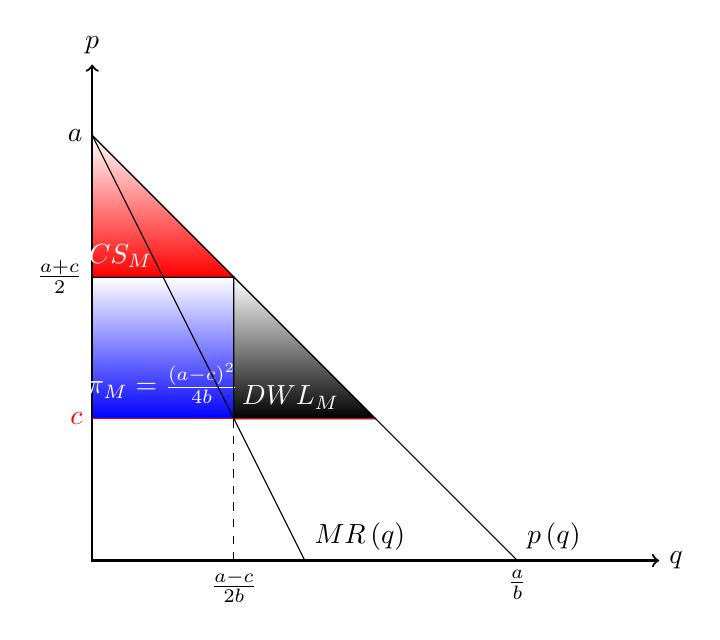
\begin{tikzpicture}[scale=0.9]
    \draw[thick,<->] (0,7) node[above] {$p$}--(0,0)--(8,0) node[right] {$q$};
    \draw (0,6) node[left] {$a$};
    \draw[top color=white,bottom color=red] (0,4) -- (2,4) -- (0,6) -- cycle;
    \draw (0.4,4.3) node[white] {$CS_M$};
    \draw[top color=white,bottom color=blue] (0,2) -- (2,2) -- (2,4) -- (0,4)
    -- cycle;
    \draw[top color=white,bottom color=black] (2,2) -- (2,4) -- (4,2) -- cycle;
    \draw (2.8,2.3) node[white] {$DWL_M$};
    \draw (1,2.5) node[white] {$\pi_M=\frac{\left( a-c \right)^2}{4b}$};
    \draw[-,red] (0,2) node[left] {$c$} (0,2)--(4,2);
    \draw[dashed,-] (0,4) node[left] {$\frac{a+c}{2}$} (0,4)--(2,4);
    \draw[dashed,-] (2,0) node[below] {$\frac{a-c}{2b}$} (2,0)--(2,4);
    \draw (6,0) node[below] {$\frac{a}{b}$};
    \draw (0,6)--(6,0);
    \draw (0,6)--(3,0);
    \draw (6,0) node[above right] {$p\left( q \right)$};
    \draw (3,0) node[above right] {$MR\left( q \right)$};
  \end{tikzpicture}
  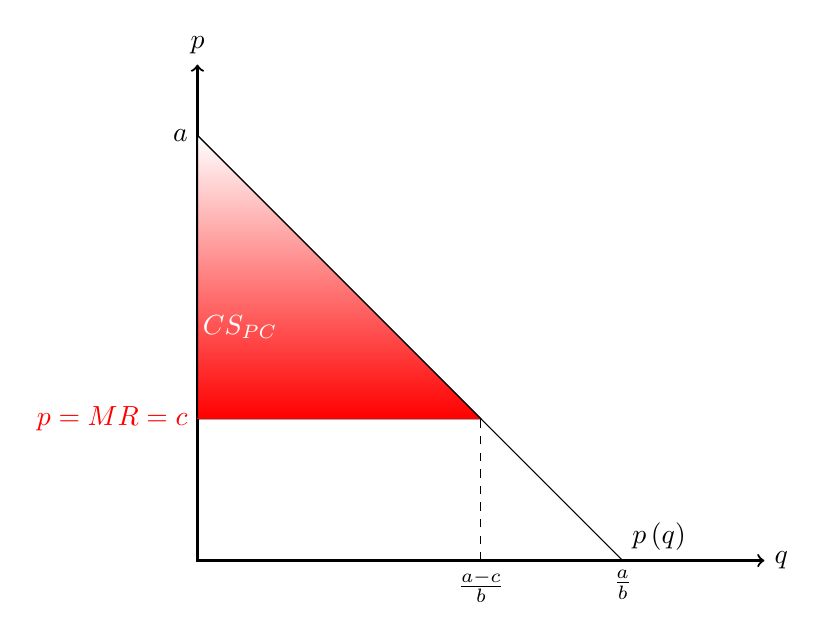
\begin{tikzpicture}[scale=0.9]
    \draw[thick,<->] (0,7) node[above] {$p$}--(0,0)--(8,0) node[right] {$q$};
    \draw (0,6) node[left] {$a$};
    \draw[top color=white,bottom color=red] (0,2) -- (4,2) -- (0,6) -- cycle;
    \draw (0.6,3.3) node[white] {$CS_{PC}$};
    \draw[-,red] (0,2) node[left] {$p=MR=c$} (0,2)--(4,2);
    \draw[dashed,-] (4,0) node[below] {$\frac{a-c}{b}$} (4,0)--(4,2);
    \draw (6,0) node[below] {$\frac{a}{b}$};
    \draw (0,6)--(6,0);
    \draw (6,0) node[above right] {$p\left( q \right)$};
  \end{tikzpicture}
\subsubsection*{Natural Monopolies}
A \emph{natural monopoly} occurs when fixed costs are very high and marginal costs are relatively small. Examples are gas delivery pipes, phone networks and subway networks. For industries like this it doesn't make sense to have firms competing with one another and duplicating the fixed cost. It is best to have a monopoly and regulate the price that it is charged (or just have the government run the firm).

For a natural monopoly, operating at $p=MC$ could result in losses to the firm.  In this case, we might regulate the natural monopoly to charge at $p=AC$, which is higher than marginal cost so there will be some deadweight loss. Alternatively, we could force the monopolist to charge at $p=MC$ and subsidize the monopolist for the loss.

\bigskip
Monopolies are more likely when the minimum efficient scale (the level of output that minimizes average costs) is similar to the level of market demand. If the mininum efficient scale is smaller than market demand, then competition is more likely to occur.
\section{Price Discrimination}
For a standard monopolist, if it lowered the price from the optimal price, it could sell additional units. However, it would have to lower the price for all units sold, so it's not worthwhile. But what if the monopolist could charge different prices for each unit? When different people pay different prices, we call this price discrimination. For this to be possible, however, it should be difficult for consumers to sell on goods to each other.

There are three different types of price discrimination:
\begin{itemize}
  \item \emph{Third-degree price discrimination} is when different people pay different prices but each unit of output sold to a given person sells for the same price (e.g.~student discounts for movie tickets).
  \item \emph{Second-degree price discrimination} is when different units of output sell for different prices but all people face the same prices (e.g.~bulk discounts, small/medium/large). This is also known as non-linear pricing.
  \item \emph{First-degree price discrimination} (also known as \emph{perfect price discrimination}) is when the monopolist sells different units of output for different prices and those prices can differ from person to person. Each person pays their willingness to pay for the products. There is no deadweight loss and no consumer surplus.
\end{itemize}

\subsubsection*{First-Degree Price Discrimination}
First degree price discrimination is more of a theoretical concept than something that exists in reality. Suppose the marginal cost of producing a good is \$2. One individual may be willing to pay \$5 for the first unit, and \$3 for the second unit and \$1 for the third unit. Another individual may be willing to pay \$3 for the first unit and \$1 for the second unit. What a perfect price discriminating monopolist would do is charge the first person \$8 for 2 units and the second person \$3 for one unit.

Under perfect price discrimination, each consumer pays their willingness to pay for each unit, as long as their willingness to pay exceeds marginal cost. Therefore there is no consumer surplus as the consumer surplus for each unit is the willingness to pay minus the price. The producer surplus, on the other hand, is very large as for each unit the producer surplus is $p-MC$. Therefore the producer surplus is the whole triangle above marginal cost, if demand is linear:

\begin{center}
  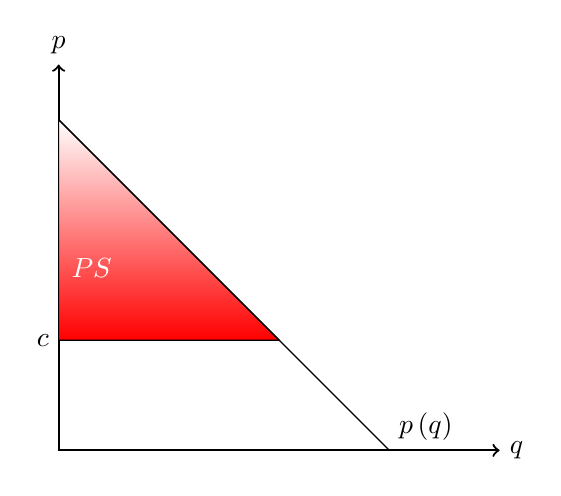
\begin{tikzpicture}[scale=0.7]
    \draw[thick,<->] (0,7) node[above] {$p$}--(0,0)--(8,0) node[right] {$q$};
    \draw[top color=white,bottom color=red] (0,2) -- (4,2) -- (0,6) -- cycle;
    \draw (0.6,3.3) node[white] {$PS$};
    \draw[-] (0,2) node[left] {$c$} (0,2)--(4,2);
    \draw (0,6)--(6,0);
    \draw (6,0) node[above right] {$p\left( q \right)$};
  \end{tikzpicture}
\end{center}

Since there is never a case where the willingness to pay exceeds the marginal cost when the product isn't bought and sold, there is no deadweight loss. A situation with a perfect-price discriminating monopolist is Pareto efficient (although not fair on the consumers). The reason this doesn't exist in reality is because it's very hard to ascertain someone's willingness to pay.


\subsubsection*{Second-Degree Price Discrimination}
Second-degree price discrimination is when different units of output
sell for different prices but all people face the same prices (e.g.~bulk
discounts). The monopolist is not able give different people different prices, as they cannot tell them apart. An example is business class and economy class in an airline. The monopolist could in principle charge people wearing suits and carrying briefcases more than people wearing shorts and sandals, but after a while the businesspeople will start to wear shorts and pack their suits in their suitcases. What the airline can do, however, is have different packages (high quality and low quality) and get the travelers to \emph{self-select} into the correct package.

\medskip
\par\noindent{\emph{Example:}}\par
There are two types of flight passengers, equal in number: business ($B$) and vacationers ($V$) and there are no costs. The monopolist cannot charge different people different prices but will offer different packages (price-quality pairs) to each customer. The monopolist chooses the price-quality pairs such that the different groups \emph{self-select} into the price-quality pair designed for them.

Each triangle in the diagram is the same size and is equal to one for simplicity. The line $V$ below measures a vacationer's willingness to pay for an additional unit of quality and the line $B$ measures a businessperson's willingness to pay for an additional unit of quality. At $q_L$ below, a vacationer would pay up to $B+E+F=3$ for a plane ticket. At the same quality, a businessperson would pay $A+B+C+E+F=5$.

The monopolist can choose between three qualities $q_L$, $q_M$ and $q_H$ and give each a price. The goal for the monopolist is to choose two qualities and two prices for those qualities to maximize profits. If the monopolist was able to tell the two consumers apart, it would like to sell to the vacationers a medium-quality package $q_M$ at the price of their full willingness to pay for it: $B+E+F+G=4$. It would sell a high-quality package $q_H$ to the businesspeople at their full willingness to pay for it: $A+B+C+D+E+F+G+H+I=9$. So it makes 4 from the vacationers and 9 from the businesspeople in this ideal case (13 overall).

But if the monopolist can't tell them apart, what the businesspeople will do is dress in shorts and sandals and buy the medium-quality package $q_M$ for $B+E+F+G=4$. They will get a positive consumer surplus from this equal to the area below their willingness-to-pay curve minus the price: $A+C+D+H=4$. The monopolist will only ever sell the $q_M$ package and make $B+E+F+G=4$ from every consumer (4 from vacationers and 4 from businesspeople).

One strategy the monopolist can do is not to charge so much for $q_H$. If they left the businesspeople with the same surplus as if they bought the $q_M$ package, they will be indifferent between the two packages (and we can assume that when indifferent they choose the higher-quality package). The monopolist would need to charge $B+E+F+G+I=5$ instead of the full triangle. This leaves the businesspeople with a surplus of $A+C+D+H=4$, the same as what they would get from buying $q_M$. The monopolist gets profits $B+E+F+G=4$ from the vacationers and $B+E+F+G+H=5$ from the businesspeople (4 from vacationers and 5 from businesspeople).

But is this the best the monopolist can do? Economy class in airlines has been getting worse and worse so you might guess the optimal thing to do is to sell the vacationers a really crappy package. Suppose you made two packages, $q_L$ and $q_H$. We want the vacationers to buy $q_L$ and the businesspeople to buy $q_H$. We will charge the vacationers their full willingness to pay, which is $B+E+F=3$. If a businessperson bought this package, they would get surplus $A+C=2$. Therefore when choosing the price for the high quality package $q_H$, the monopolist needs to ensure that the businesspeople get at least a surplus $A+C=2$ so they don't buy the low quality package. So it will charge $B+D+E+F+G+H+I=7$.

The profits for the monopolist is $B+E+F=3$ from vacationers and $B+D+E+F+G+H+I=7$ from businesspeople. Therefore with $q_L$ and $q_H$ the monopolist can make 3+7=10 and with $q_M$ and $q_H$ it was only able to make 4+5=9. However, this is less than the ideal case where the monopolist can tell consumers apart where it can make 13. Compared to the perfect price discrimination case, it loses 1 from the vacationers ($G$) and 2 from the businesspeople ($A+C$).

\begin{center}
  \begin{tikzpicture}[scale=0.8]
    \draw[thick,<->] (0,9) node[above] {$WTP$}--(0,0)--(9,0) node[below right]
    {Quality, $q$};
    \draw[dashed,-] (0,5)--(2.5,5);
    \draw[dashed,-] (5,0)--(5,2.5);
    \draw[dashed,-] (2.5,0)--(2.5,5);
    \draw[dashed,-] (0,2.5)--(5,2.5);
    \draw[dashed,-] (0,2.5)--(2.5,0);
    \draw (2.5, 0) node[below] {$q_L$};
    \draw (5, 0) node[below] {$q_M$};
    \draw (7.5, 0) node[below] {$q_H$};
    \draw (0,7.5)--(7.5,0) node[above right] {\textcolor{red}{\sl B}};
    \draw (0,5)--(5,0) node[above right] {\textcolor{red}{\sl V}};
    \draw (0.8, 6.2) node {$A$};
    \draw (1, 3.25) node {$B$};
    \draw (1.5, 4.25) node {$C$};
    \draw (3.2,3.75) node {$D$};
    \draw (0.9,0.9) node {$E$};
    \draw (2,2) node {$F$};
    \draw (3,1) node {$G$};
    \draw (4,2) node {$H$};
    \draw (6,1) node {$I$};
  \end{tikzpicture}
\end{center}
So the monopolist is purposefully making economy class really bad to stop the high willingness to pay consumers from being tempted by it, at the detriment of the low willingness to pay consumers.
\subsubsection*{Third-degree price discrimination}
\vspace{-1mm}
\emph{Third-degree price discrimination} is when different people pay different
prices but each unit of output sold to a given person sells for the same price
(e.g.~student discounts for movie tickets).

For example, let $p_1\left(q_1  \right)$ and $p_2\left( q_2 \right)$ be the
inverse demand curves for two types of people (e.g.~professionals and
students). If the monopolist can price discriminate the monopolist's problem
is:
\vspace{-2mm}
\[
  \underset{\left\{q_1,q_2  \right\}}{\max}\;p_1\left( q_1 \right)q_1+ p_2\left(
  q_2 \right)q_2 - c\left( q_1+q_2 \right)
\]
The first-order conditions are $MR_1\left( q_1 \right)=MC\left( q_1+q_2
\right)$ and $MR_2\left( q_2 \right)=MC\left( q_1+q_2 \right)$. These are two
equations with two unknowns ($q_1$ and $q_2$).
The monopolist should choose quantities to make the marginal revenue
from both groups the same: $MR_1\left(  q_1 \right)=MR_2\left( q_2 \right)$.

Suppose the monopolist optimally chose to charge a higher price to group 1. Then since $MR=p\left( q \right)\left[ 1-\frac{1}{\left| \varepsilon\left( q \right) \right|} \right]$:
\[
  p_1\left( q_1 \right)>p_2\left( q_2 \right) \;\;\;\Longrightarrow\;\;\;
  \left[ 1-\frac{1}{\left| \varepsilon\left( q_1 \right) \right|} \right]<
  \left[ 1-\frac{1}{\left| \varepsilon\left( q_2 \right) \right|} \right]
  \;\;\;\Longrightarrow\;\;\;
  \frac{1}{\left| \varepsilon\left( q_1 \right) \right|}< \frac{1}{\left| \varepsilon\left( q_2 \right) \right|}
  \;\;\;\Longrightarrow\;\;\;
  \left| \varepsilon\left( q_2 \right) \right|>\left| \varepsilon\left( q_1 \right) \right|
\]
The monopolist will charge a higher price to the \emph{less elastic} group.

\medskip
\par\noindent\emph{Example}\par
$D_1\left( p_1 \right)=100-p1$ and $D_2\left( p_2 \right)=100-2p_2$. Marginal cost is $20$. The inverse demand curves are $p_1\left( q_1 \right)=100-q_1$ and $p_2\left( q_2 \right)=50-\frac{q_2}{2}$.

The marginal revenue functions are $MR_1\left( q_1 \right)=100-2q_1$ and $MR_2\left(q_2  \right)=50-q_2$. Setting $MR_1=MC$ gives $100-2q_1=20$ so $q_1=40$. Setting $MR_2=MC$ gives $50-q_2=20$ so $q_2=30$. The prices are then $p_1=60$ and $p_2=35$. Profit is then $60\times 40 + 35 \times 30 = \$3,450$.

Suppose you couldn't price discriminate? The total demand is then $D\left( p \right)=D_1\left( p \right)+D_2\left( p \right)=100-p + 100- 2p = 200 - 3p$. The inverse demand is then $p\left( q \right)=\frac{200}{3}-\frac{q}{3}$. Marginal revenue is $MR\left( q \right)=\frac{200}{3}-\frac{2q}{3}$. Setting $MR\left( q \right)=MC\left( q \right)$ gives $\frac{200}{3}-\frac{2q}{3}=20$ so $q=70$. Therefore price is $p=\frac{200}{3}-\frac{70}{3}=\frac{130}{3}=43\frac{1}{3}$. Profits are then $70\times 43\frac{1}{3}=\$3,033.33$, smaller than under price discrimination.
\subsubsection*{Bundling}
If different people value different products differently, monopolists are also able to \emph{bundle} products together to increase profits. Suppose there are two types of consumers, journalists and accountants, equal in number. There are two desktop applications, Word and Excel. Journalists and accountants need both software but journalists find Word more useful and accountants find Excel more useful. Their willingness to pay for two desktop applications are:

\begin{center}
  \begin{tabular}{l|l|l}
    & Word & Excel \\ \hline\hline
    Journalist &  120 & 100 \\ \hline
    Accountant &  100 & 120 \\ \hline\hline
  \end{tabular}
\end{center}
The monopolist's marginal cost is zero (in reality, the marginal cost of software is actually zero).

Charging 120 for each would exclude half the market so charging 100 for each is better. However, the monopolist can do even better than that. What if they bundled the two applications into an ``Office Suite'' for \$220? Both consumers would still be willing to buy the bundle but now they get zero surplus.
\subsubsection*{Two-Part Tariffs}
There is a theme park that charges for entry and then also charges for each ride. Suppose everyone has the same demand curve for rides at the theme park. If the monopolist only charged for rides, it would earn profits as it normally does and the profits is the blue box on the left diagram. However, suppose the monopolist charged a price for rides equal to marginal cost. The consumer surplus would be the whole red triangle on the right diagram. What the monopolist can do is just set the entry price equal to that consumer surplus and steal the entire consumer surplus. If the marginal cost is close to zero, you may see places in real life following this strategy where there is only an entry cost and the price for a ride is zero.

\begin{center}
  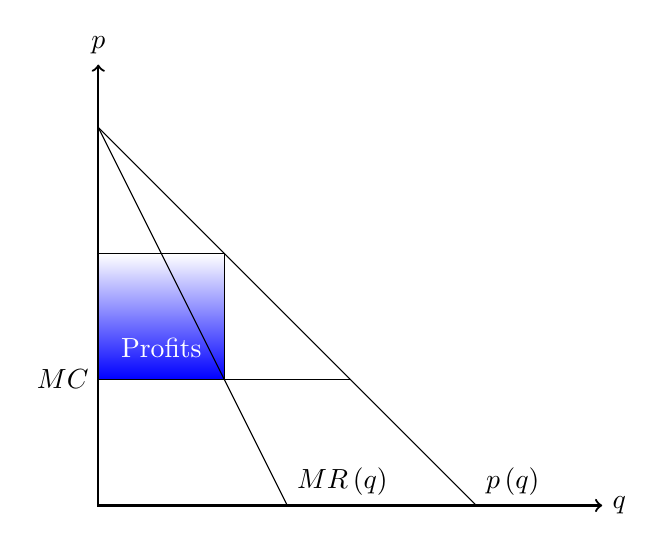
\begin{tikzpicture}[scale=0.8]
    \draw[thick,<->] (0,7) node[above] {$p$}--(0,0)--(8,0) node[right] {$q$};
    \draw[top color=white,bottom color=blue] (0,2) -- (2,2) -- (2,4) -- (0,4)
    -- cycle;
    \draw (1,2.5) node[white] {Profits};
    \draw[-] (0,2) node[left] {$MC$} (0,2)--(4,2);
    \draw (0,6)--(6,0);
    \draw (0,6)--(3,0);
    \draw (6,0) node[above right] {$p\left( q \right)$};
    \draw (3,0) node[above right] {$MR\left( q \right)$};
  \end{tikzpicture}
  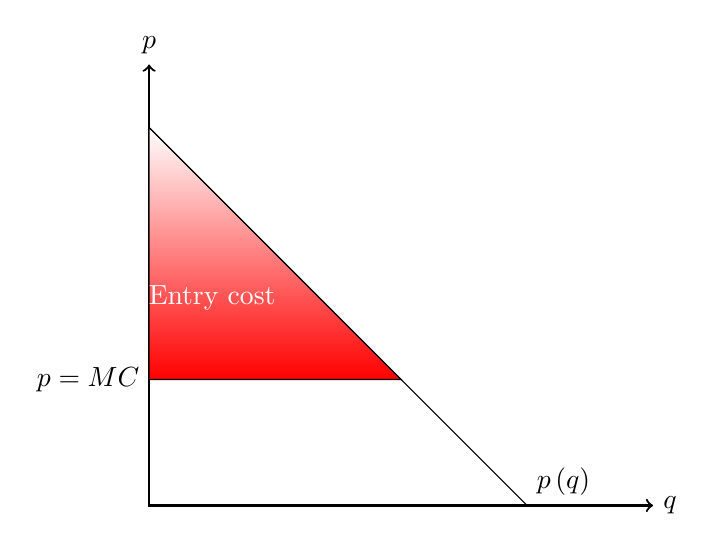
\begin{tikzpicture}[scale=0.8]
    \draw[thick,<->] (0,7) node[above] {$p$}--(0,0)--(8,0) node[right] {$q$};
    \draw[top color=white,bottom color=red] (0,2) -- (4,2) -- (0,6) -- cycle;
    \draw (1.0,3.3) node[white] {Entry cost};
    \draw[-] (0,2) node[left] {$p=MC$} (0,2)--(4,2);
    \draw (0,6)--(6,0);
    \draw (6,0) node[above right] {$p\left( q \right)$};
  \end{tikzpicture}
\end{center}


\section{Game Theory}
Game theory studies the strategic interaction between players
\subsubsection*{The Normal Form Representation of a Game (Payoff Matrix)}
\begin{itemize}
  \item A \emph{payoff matrix} shows the payoffs for each player given their
    action and the action of the other player.
    \begin{center}
      \begin{tabular}{llcc}
        & & \multicolumn{2}{c}{\emph{Firm B}} \\
        & & High price & Low price \\ \cline{3-4}
        \multirow{2}{*}{\emph{Firm A}} & High price & \multicolumn{1}{|c|}{5, 5} & \multicolumn{1}{c|}{0, 10} \\ \cline{3-4}
        & Low price & \multicolumn{1}{|c|}{10, 0} & \multicolumn{1}{c|}{1, 1} \\ \cline{3-4}
      \end{tabular}
    \end{center}
  \item The left number is the payoff for the left player, the right number is the payoff for the top player.
\end{itemize}
\subsubsection*{Strategies}
\begin{itemize}
  \item A \emph{strategy} is what a player will do given every action of the other player. Your strategy is like the instructions you would give to a robot playing the game for you.
   \item A player has a \emph{dominant strategy} if one action is optimal for
     that player no matter what the other player does. In the example above, playing ``Low price'' is a \emph{dominant strategy} for both players.
  \item We say a particular strategy of a player is a \emph{dominated strategy}
    if one action gives a higher payoff than the dominated strategy, no matter
    what the other player does. In the example above, ``High price'' is dominated for both players.
\end{itemize}
\subsubsection*{Nash Equilibrium}
\begin{itemize}
  \item We want to be able to predict what the outcome of a game is.
  \item If both players have a dominant strategy, we would predict that that will be the outcome of the game (in the example above, both firms play ``Low price'').
  \item However, not every game has dominant strategies. Consider the following example where two people had agreed to meet at a classical music concert but both of their phones died. Going alone to a concert gives them zero payoff, but conditional on going together Andy prefers Bach and Betty prefers Stravinsky:
    \begin{center}
      \begin{tabular}{llcc}
        & & \multicolumn{2}{c}{\emph{Betty}} \\
        & & Bach & Stravinsky \\ \cline{3-4}
        \multirow{2}{*}{\emph{Andy}} & Bach & \multicolumn{1}{|c|}{2, 1} & \multicolumn{1}{c|}{0, 0} \\ \cline{3-4}
        & Stravinksky & \multicolumn{1}{|c|}{0, 0} & \multicolumn{1}{c|}{1, 2} \\ \cline{3-4}
      \end{tabular}
    \end{center}
  \item In the Bach and Stravinsky example, both player's optimal strategies is to go to the same concert as the other person. For example, Andy's best response to Betty playing ``Bach'' is also to play ``Bach'' and Andy's best response to Betty playing ``Stravinsky'' is also to play ``Stravinsky''. We can mark each player's \emph{best response} to the other player's action with a $\star$:
    \begin{center}
      \begin{tabular}{llcc}
        & & \multicolumn{2}{c}{\emph{Betty}} \\
        & & Bach & Stravinsky \\ \cline{3-4}
        \multirow{2}{*}{\emph{Andy}} & Bach & \multicolumn{1}{|c|}{2$^\star$, 1$^\star$} & \multicolumn{1}{c|}{0, 0} \\ \cline{3-4}
        & Stravinksky & \multicolumn{1}{|c|}{0, 0} & \multicolumn{1}{c|}{1$^\star$, 2$^\star$} \\ \cline{3-4}
      \end{tabular}
    \end{center}
  \item If two players' best responses overlap (one square has two $\star$s), then we call it a \emph{Nash Equilibrium}. More generally, a pair of strategies is a \emph{Nash Equilibrium} if both players' choices are optimal given the other player's choice. No player has any incentive to unilaterally deviate from a Nash Equilibrium. In the example above $\left( Bach, Bach \right)$ and $\left( Stravinsky, Stravinsky \right)$ are two Nash equilibria of the game.
  \item The best response functions don't always overlap. Consider the following example of a striker and a goalkeaper during a penalty shootout in football. If the goalkeeper jumps in the correct direction, he will save the ball. If not, the striker scores (keep in mind, since the two players are facing each other, left and right are the opposite location for each). The best responses don't overlap in any case here:
    \begin{center}
      \begin{tabular}{llcc}
        & & \multicolumn{2}{c}{\emph{Goalkeeper}} \\
        & & Jump Left & Jump Right \\ \cline{3-4}
        \multirow{2}{*}{\emph{Striker}} & Shoot Left & \multicolumn{1}{|c|}{1$^\star$, -1} & \multicolumn{1}{c|}{-1, 1$^\star$} \\ \cline{3-4}
        & Shoot Right & \multicolumn{1}{|c|}{-1, 1$^\star$} & \multicolumn{1}{c|}{1$^\star$, -1} \\ \cline{3-4}
      \end{tabular}
    \end{center}
  \item As an aside, a game in which the total payoffs in each outcome sum to zero is called a \emph{zero-sum game}.
\end{itemize}
\subsubsection*{Mixed Strategies}
A \emph{pure strategy} is when the agent makes one choice an sticks to it. A \emph{mixed strategy} is when the agent randomizes between two or more strategies.

In the penalty kick example, there was no pure strategy Nash equilibrium (PSNE). However, there is a mixed strategy Nash equilibrium (MSNE).

Suppose the striker played ``Left'' with probability $p$ and ``Right'' with probability $1-p$. Similarly suppose the goalkeeper player ``Left'' with probability $q$ and ``Right'' with probability $1-q$. If the striker is optimally playing a mixed strategy, then it must be the case that given the goalkeeper's randomization, the striker doesn't prefer one strategy over another in expectation. Therefore the expected value from either strategy must be the same, given the other player's randomization. So:
\[
  \underbrace{1\times q + \left( -1 \right)\times \left( 1-q \right)}_{\text{Expected payoff from shooting ``Left''}}=
  \underbrace{\left( -1 \right)\times q + 1\times \left( 1-q \right)}_{\text{Expected payoff from shooting ``Right''}}
\]
Solving for $q$:
\[q-\left( 1-q \right)=-q + 1-q \;\;\;\Longrightarrow\;\;\;
  2q-1=1-2q\;\;\;\Longrightarrow\;\;\;
  4q=2\;\;\;\Longrightarrow\;\;\;
  q=\frac{1}{2}
\]
So the goalkeeper must be randomizing with probability $\frac{1}{2}$ for the striker to be indifferent between shooting left and right. This makes sense, if the goalkeeper was playing ``Left'' more often than ``Right'', then the striker would shoot ``Left'' all the time and score more often. Similarly, if the goalkeeper was playing ``Right'' more often than ``Left'', then the striker would shoot ``Right'' all the time and score more often.

We can do the same for the goalkeeper:
\[
  \underbrace{\left( -1 \right)\times p + 1\times \left( 1-p \right)}_{\text{Expected payoff from jumping ``Left''}}=
  \underbrace{1\times p + \left( -1 \right)\times \left( 1-p \right)}_{\text{Expected payoff from jumping ``Right''}}
\]
Solving for $p$ yields $p=\frac{1}{2}$ like above. Both players flip a coin and shoot and jump randomly left and right in equilibrium. Both players get an expected payoff of 0. The MSNE is $p=\frac{1}{2}$ and $q=\frac{1}{2}$.
\bigskip
\par\noindent\emph{Bach or Stravinsky example:}
The Bach or Stravinsky example also has a MSNE. Andy goes to Bach with probability $p$ and Betty goes to Bach with probability $q$. Andy is indifferent between Bach and Stravinsky if:
\[
  2q + 0\times \left( 1-q \right)=0\times q + 1\times \left( 1-q \right)
\]
Solving yields $q=\frac{1}{3}$. Betty is indifferent between Bach and Stravinsky if:
\[
  1\times p + 0\times \left( 1-p \right)=0\times p + 2\left( 1-p \right)
\]
Solving yield $p=\frac{2}{3}$. So there is a MSNE with $p=\frac{2}{3}$ and $q=\frac{1}{3}$.

\subsubsection*{Sequential Games}
In the previous examples, both players moved at the same time. The goalkeeper and the striker had to choose which direction to jump and shoot at the same time. We will now consider what happens when players take turns. Consider the following example. Player 1 moves first and can go either $L$  or $R$. Player 2 can then do either $A$ or $B$:

\begin{center}
  \begin{tikzpicture}[scale=1.5,font=\footnotesize]
    \tikzstyle{solid node}=[circle,draw,inner sep=1.5,fill=black]
    \tikzstyle{hollow node}=[circle,draw,inner sep=1.5]
    \tikzstyle{level 1}=[level distance=15mm,sibling distance=3.5cm]
    \tikzstyle{level 2}=[level distance=15mm,sibling distance=1.5cm]
    \tikzstyle{level 3}=[level distance=15mm,sibling distance=1cm]
    \node(0)[hollow node,label=above:{$P1$}]{}
    child{node[solid node,label=above left:{$P2$}]{}
      child{node[label=below:{$(1,9)$}]{} edge from parent node[left]{$A$}}
      child{node[label=below:{$(1,9)$}]{} edge from parent node[left]{$B$}}
      edge from parent node[left,xshift=-5]{$L$}
    }
    child{node[solid node,label=above right:{$P2$}]{}
      child{node[label=below:{$(0,0)$}]{} edge from parent node[left]{$A$}}
      child{node[label=below:{$(2,1)$}]{} edge from parent node[left]{$B$}}
      edge from parent node[left,xshift=-5]{$R$}
    };
  \end{tikzpicture}
\end{center}
This is the \emph{extensive form} of a game. It is a representation of the game showing the order in which the players move. We can also write the game in \emph{normal form} like we did before:
    \begin{center}
      \begin{tabular}{llcc}
        & & \multicolumn{2}{c}{\emph{Player 2}} \\
        & & $A$& $B$\\ \cline{3-4}
        \multirow{2}{*}{\emph{Player 1}} & $L$& \multicolumn{1}{|c|}{1$^\star$, 9$^\star$} & \multicolumn{1}{c|}{1, 9$^\star$} \\ \cline{3-4}
        & $R$ & \multicolumn{1}{|c|}{0, 0} & \multicolumn{1}{c|}{2$^\star$, 1$^\star$} \\ \cline{3-4}
      \end{tabular}
    \end{center}
    This game has two pure strategy Nash equilibria $\left( L,A \right)$ and $\left( R,B \right)$. But does $\left( L,A \right)$ make any sense if Player 1 moves first? If Player 1 moves first, he can avoid getting the payoff of 1 by moving $R$ and thereby forcing player 2 to play $B$ (as $B$ gives Player 2 a payoff of 1 and $A$ gives player 2 a payoff of 0). Since the definition of Nash equilibrium can lead us to unreasonable predictions in sequential games we define a new concept of equilibrium called \emph{Subgame Perfect Nash Equilibria} (SPNE).

    We can find SPNE of extensive form games using \emph{backward induction}. First you start at the end of the game and mark off what the optimal thing a player would do if the game ended up there. If Player 1 played $L$, Player 2 is indifferent between $A$ and $B$. But in any case, the payoffs are the same. If Player 1 played $R$, Player 2 would play $B$. We can therefore delete the node where Player 2 plays $A$ after Player 1 plays $R$:
\begin{center}
  \begin{tikzpicture}[scale=1.5,font=\footnotesize]
    \tikzstyle{solid node}=[circle,draw,inner sep=1.5,fill=black]
    \tikzstyle{hollow node}=[circle,draw,inner sep=1.5]
    \tikzstyle{level 1}=[level distance=15mm,sibling distance=3.5cm]
    \tikzstyle{level 2}=[level distance=15mm,sibling distance=1.5cm]
    \tikzstyle{level 3}=[level distance=15mm,sibling distance=1cm]
    \node(0)[hollow node,label=above:{$P1$}]{}
    child{node[label=below left:{$\left( 1,9 \right)$}]{}
    edge from parent node[left,xshift=-5]{$L$}
    }
    child{node[label=below right:{$\left( 2,1 \right)$}]{}
    edge from parent node[right,xshift=5]{$R$}
    };
  \end{tikzpicture}
\end{center}
Player 1 will now choose $R$ as 2 is greater than 1. The SPNE of this game is $\left( R,B \right)$.

Consider another example:
\begin{center}
 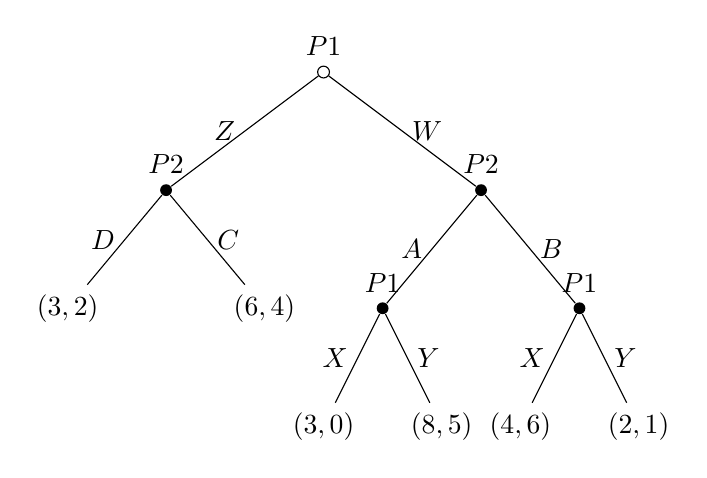
\begin{tikzpicture}[thin,
      level 1/.style={sibling distance=40mm},
      level 2/.style={sibling distance=25mm},
      level 3/.style={sibling distance=15mm},
      every circle node/.style={minimum size=1.5mm,inner sep=0mm}]
      \node[circle,draw,label=above:$P1$] (root) {}
        child { node [circle,fill,label=above:$P2$] {}
          child {
            node {$\left(3,2\right)$}
            edge from parent
              node[left] {$D$}}
          child {
            node {$\left(6,4\right)$}
            edge from parent
              node[right] {$C$}}
          edge from parent
            node[left] {$Z$}}
        child { node [circle,fill,label=above:$P2$] {}
          child {
            node[circle,fill,label=above:$P1$] (node-A) {}
              child {
                node {$\left(3,0\right)$}
                edge from parent
                  node[left] {$X$}}
              child {
                 node {$\left(8,5\right)$}
                 edge from parent
                   node[right] {$Y$}}
              edge from parent
                node[left] {$A$}}
          child { 
            node[circle,fill,label=above:$P1$] (node-B) {}
              child {
                node {$\left(4,6\right)$}
                edge from parent
                  node[left] {$X$}}
              child {
                node {$\left(2,1\right)$}
                 edge from parent
                   node[right] {$Y$}}
              edge from parent
                node[right] {$B$}}
           edge from parent
             node[right] {$W$}};
    \end{tikzpicture}
\end{center}
We can solve it via backward induction. What will Player 1 do at the end of the game? It will play $Y$ at the left node (8 is better than 3) and $X$ at the right node (4 is better than 2). We can highlight those actions and delete the other actions:
\begin{center}
 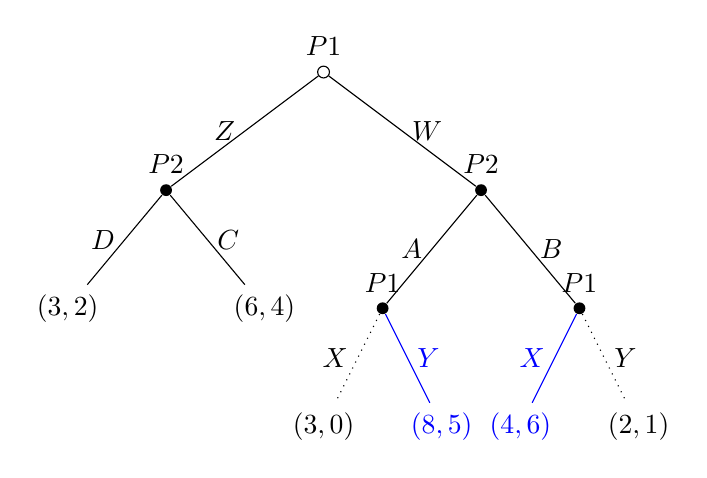
\begin{tikzpicture}[thin,
      level 1/.style={sibling distance=40mm},
      level 2/.style={sibling distance=25mm},
      level 3/.style={sibling distance=15mm},
      every circle node/.style={minimum size=1.5mm,inner sep=0mm}]
      \node[circle,draw,label=above:$P1$] (root) {}
        child { node [circle,fill,label=above:$P2$] {}
          child {
            node {$\left(3,2\right)$}
            edge from parent
              node[left] {$D$}}
          child {
            node {$\left(6,4\right)$}
            edge from parent
              node[right] {$C$}}
          edge from parent
            node[left] {$Z$}}
        child { node [circle,fill,label=above:$P2$] {}
          child {
            node[circle,fill,label=above:$P1$] (node-A) {}
              child {
                node {$\left(3,0\right)$}
                edge from parent[dotted]
                  node[left] {$X$}}
              child {
                 node[blue] {$\left(8,5\right)$}
                 edge from parent[blue]
                   node[right] {$Y$}}
              edge from parent
                node[left] {$A$}}
          child { 
            node[circle,fill,label=above:$P1$] (node-B) {}
              child {
                node[blue] {$\left(4,6\right)$}
                edge from parent[blue]
                  node[left] {$X$}}
              child {
                node {$\left(2,1\right)$}
                edge from parent[dotted]
                   node[right] {$Y$}}
              edge from parent
                node[right] {$B$}}
           edge from parent
             node[right] {$W$}};
    \end{tikzpicture}
\end{center}
What will player 2 do now? At the very left it will choose $C$ over $D$ as 4 is greater than 2. On the right it will choose $B$ over $A$ as 6 is better than 5 (note that we deleted the other possibilities as we know player 1 won't play them).
\begin{center}
 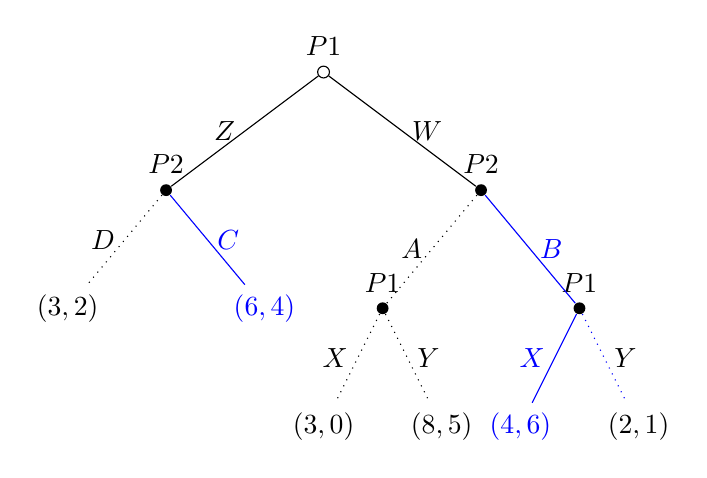
\begin{tikzpicture}[thin,
      level 1/.style={sibling distance=40mm},
      level 2/.style={sibling distance=25mm},
      level 3/.style={sibling distance=15mm},
      every circle node/.style={minimum size=1.5mm,inner sep=0mm}]
      \node[circle,draw,label=above:$P1$] (root) {}
        child { node [circle,fill,label=above:$P2$] {}
          child {
            node {$\left(3,2\right)$}
            edge from parent[dotted]
              node[left] {$D$}}
          child {
            node[blue] {$\left(6,4\right)$}
            edge from parent[blue]
              node[right] {$C$}}
          edge from parent
            node[left] {$Z$}}
        child { node [circle,fill,label=above:$P2$] {}
          child {
            node[circle,fill,label=above:$P1$] (node-A) {}
              child {
                node {$\left(3,0\right)$}
                edge from parent[dotted]
                  node[left] {$X$}}
              child {
                 node {$\left(8,5\right)$}
                 edge from parent[dotted]
                   node[right] {$Y$}}
                   edge from parent[dotted]
                node[left] {$A$}}
          child { 
            node[circle,fill,label=above:$P1$] (node-B) {}
              child {
                node[blue] {$\left(4,6\right)$}
                edge from parent[blue]
                  node[left] {$X$}}
              child {
                node {$\left(2,1\right)$}
                edge from parent[dotted]
                   node[right] {$Y$}}
                   edge from parent[blue]
                node[right] {$B$}}
           edge from parent
             node[right] {$W$}};
    \end{tikzpicture}
\end{center}
Now we are at the beginning of the game. What will Player 1 do? If it plays $Z$ it will get 6. If it plays $W$ it will get 4. So it will play $Z$ as 6 is better than 4:
\begin{center}
 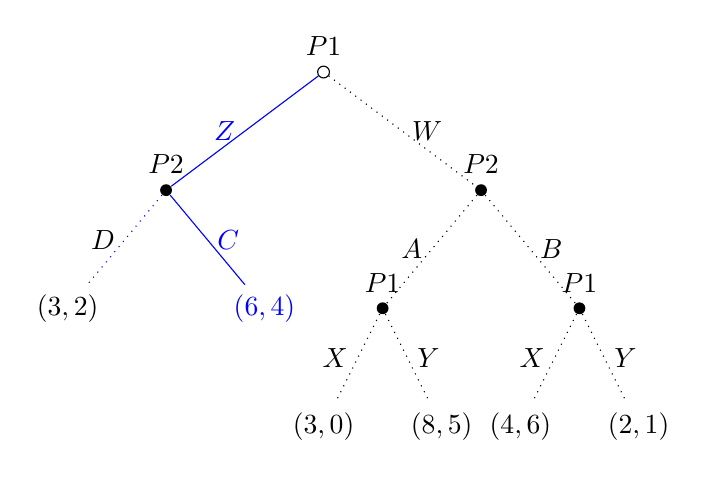
\begin{tikzpicture}[thin,
      level 1/.style={sibling distance=40mm},
      level 2/.style={sibling distance=25mm},
      level 3/.style={sibling distance=15mm},
      every circle node/.style={minimum size=1.5mm,inner sep=0mm}]
      \node[circle,draw,label=above:$P1$] (root) {}
        child { node [circle,fill,label=above:$P2$] {}
          child {
            node {$\left(3,2\right)$}
            edge from parent[dotted]
              node[left] {$D$}}
          child {
            node[blue] {$\left(6,4\right)$}
            edge from parent[blue]
              node[right] {$C$}}
              edge from parent[blue]
            node[left] {$Z$}}
        child { node [circle,fill,label=above:$P2$] {}
          child {
            node[circle,fill,label=above:$P1$] (node-A) {}
              child {
                node {$\left(3,0\right)$}
                edge from parent[dotted]
                  node[left] {$X$}}
              child {
                 node {$\left(8,5\right)$}
                 edge from parent[dotted]
                   node[right] {$Y$}}
                   edge from parent[dotted]
                node[left] {$A$}}
          child { 
            node[circle,fill,label=above:$P1$] (node-B) {}
              child {
                node {$\left(4,6\right)$}
                edge from parent[dotted]
                  node[left] {$X$}}
              child {
                node {$\left(2,1\right)$}
                edge from parent[dotted]
                   node[right] {$Y$}}
                   edge from parent[dotted]
                node[right] {$B$}}
                edge from parent[dotted]
             node[right] {$W$}};
    \end{tikzpicture}
\end{center}
In the SPNE of this game, player 1 plays $Z$ at the beginning and player 2 plays $C$.

\section{Oligopoly}
Oligopoly comes from Ancient Greek: \emph{olígos} means ``few'' and \emph{polein} means sell. Therefore it means ``few sellers''. In oligopoly there are only a few firms so the actions of each firm affects the action of every other firm. For example, if one firm decreases price, the other firms might react by also decreasing price. For simplicity, we will only consider the 2-firm case (the algebra gets cumbersome for more firms and the intuition stays the same). We will study 3 different models: simultaneous price setting (Bertrand), simultaneous quantity setting (Cournot) and Staggered quantity setting (Stackelberg). There is another model that studies staggered price setting, but for time reasons we skip that model (it's in the book if you are interested).
\subsubsection*{Simulatenous Price Setting (Bertrand)}
If each firm has the same constant marginal cost, the equilibrium in Bertrand competition is for both firms to set $p=MC$. If a firm set $p>MC$, the other firm would undercut it. If a firm set $p<MC$ it would make a loss.
\subsubsection*{Simulatenous Quantity Setting (Cournot)}
Each firm's problem is:
\[
  \underset{q_1}{\max}\; p\left( q_1+q_2 \right)q_1 - c\left( q_1 \right)
  \;\;\;\;\;\;\;\;\;\;\;\;
  \;\;\;\;\;\;\;\;\;\;\;\;
  \underset{q_2}{\max}\; p\left( q_1+q_2 \right)q_2 - c\left( q_2 \right)
\]
The optimal choice of quantity depends on the quantity of the other firm: $q_1^\star = q_1\left( q_2 \right)$ and $q_2^\star = q_2\left( q_1 \right)$. These are the firms' \emph{reaction functions}. These are the best response functions for each firm. In equilibrium, both reaction curves must be satisfied. Let's take a look at an example with linear demand and costs.

With $p\left( q \right)=a-bq$ and $c\left( q \right)=cq$, the profit for firm 1 is:
\[
  \pi_1\left( q_1,q_2 \right)=\left[ a-b\left( q_1+q_2 \right) \right]q_1 - cq_1=aq_1 - bq_1^2 -b q_1q_2 -cq_1 = \left( a-c \right)q_1 - bq_1^2 - bq_1q_2
\]
For firm 2:
\[
   \pi_1\left( q_1,q_2 \right)=\left[ a-b\left( q_1+q_2 \right) \right]q_2 - cq_2=aq_2 - bq_2^2 -b q_1q_2 -cq_2 = \left( a-c \right)q_2 - bq_2^2 - bq_1q_2
\]
Firm 1's reaction curve is $q_1$ as a function of $q_2$ where $\frac{d\pi_1\left( q_1 \right)}{dq_1}=0$, i.e.~profits are maximized:
\[
  a -c - 2bq_1 -bq_2 = 0 \;\;\;\Longrightarrow \;\;\; q_1\left( q_2 \right) = \frac{a-c-bq_2}{2b}
\]
Firm 2's reaction curve is $q_2$ as a function of $q_1$ where $\frac{d\pi_2\left( q_2 \right)}{dq_2}=0$:
\[
  a-c - 2bq_2 -bq_1 = 0 \;\;\;\Longrightarrow \;\;\; q_2\left( q_1 \right)= \frac{a-c-bq_1}{2b}
\]
In equilibrium the reaction curves will intersect. We can put $q_2\left( q_1 \right)$ into $q_1\left( q_2 \right)$:
\begin{align*}
  q_1&=\frac{1}{2b}\left[ a-c-\frac{1}{2}\left( a-c-bq_1 \right) \right]\\
  q_1&=\frac{a-c}{2b} -\frac{a-c}{4b} + \frac{q_1}{4}\\
  q_1-\frac{q_1}{4}&=\frac{a-c}{4b}\\
  \frac{3q_1}{4}&=\frac{a-c}{4b}\\
  q_1&=\frac{a-c}{3b}\\
\end{align*}
Similarly, $q_2=\frac{a-c}{3b}$. The total quantity produced is $q=q_1+q_2=\frac{a-c}{3b}+\frac{a-c}{3b}=\frac{2}{3}\frac{a-c}{b}$.

The profit for firm firm 1:
\begin{align*}
  \pi_1\left( q_1,q_2 \right)=&\left( a-c \right)q_1-bq_1^2 - bq_1q_2 \\
  =&\left( a-c \right)\frac{a-c}{3b} - b\left( \frac{a-c}{3b} \right)^2 - b\left( \frac{a-c}{3b} \right)^2 \\
  =& \frac{\left( a-c \right)^2}{3b}-2b\frac{\left( a-c \right)^2}{9b^2} \\
  =& 3\frac{\left( a-c \right)^2}{9b}-2\frac{\left( a-c \right)^2}{9b} \\
  =& \frac{\left( a-c \right)^2}{9b}
\end{align*}
The profit for firm 2 is also $\frac{\left( a-c \right)^2}{9b}$.

Graphically, the two reaction curves are as follows:
\begin{center}
  \begin{tikzpicture}[scale=1]
    \draw [thick,<->] (0,7) node [above] {$q_2$} --(0,0)--(7,0) node [right] {$q_1$};
    \node [below] at (2.35,0) {$\frac{a-c}{3b}$};
    \node [left] at (0,5.8) {$\frac{a-c}{b}$};
    \node [left] at (0,3.8) {$\frac{a-c}{2b}$};
    \node [below] at (5.8,0) {$\frac{a-c}{b}$};
    \node [below] at (3.8,0) {$\frac{a-c}{2b}$};
    \node [left] at (0,2.1) {$\frac{a-c}{3b}$};
    \node [above right] at (2.35,2.1) {$\left( q_1^\star,q_2^\star \right)$};
    \draw [dashed] (0, 2.1) -- (2.35,2.1);
    \draw [dashed] (2.35, 0) -- (2.35,2.1);
    \node [above right] at (0.8,4.3) {$q_1\left( q_2 \right)$};
    \node [above right] at (4.0,1.1) {$q_2\left( q_1 \right)$};
    \draw (0,3.5)--(5.8,0);
    \draw (0,5.7)--(3.7,0);
  \end{tikzpicture}
\end{center}
Firm 1's reaction curve $q_1\left( q_2 \right)$ gives the optimal amount to produce in response to any output of firm 2. If firm 2 produces zero output, firm 1 will optimally react by producing $\frac{a-c}{2b}$, the monopolist output. If firm 2 produces the perfectly competitive output $\frac{a-c}{b}$, then firm 1 will optimally react by producing nothing (as any increase in quantity will lead the price to be lower than marginal cost). If firm 2 produces $\frac{a-c}{3b}$, then firm 1 will optimally react by producing $\frac{a-c}{3b}$ as well. In equilibrium, both firms won't want to react to each other's output, which is at $\frac{a-c}{3b}$. Since neither firm wants to deviate at this out, it is a Nash equilibrium.

A firm's \emph{isoprofit curve} shows the different quantity combinations for both firms $\left( q_1,q_2 \right)$ that give the same amount of profits. Firm 1's profits are:
\[
  \pi_1\left( q_1,q_2 \right)=\left( a-c \right)q_1-bq_1^2 - bq_1q_2
\]
At a fixed profit level $\bar{\pi}$, we can solve for $q_2$ to find the isoprofit function:
\begin{align*}
  \bar{\pi} &= \left( a-c \right)q_1 - bq_1^2 -bq_1q_2 \\
  bq_1 q_2 &= \left( a-c \right)q_1 - bq_1^2 -\bar{\pi} \\
  q_2 &= \frac{a-c}{b}-q_1 - \frac{\bar{\pi}}{bq_1}
\end{align*}
Graphically, the isoprofit curves for firm 1 look as follows:
\begin{center}
  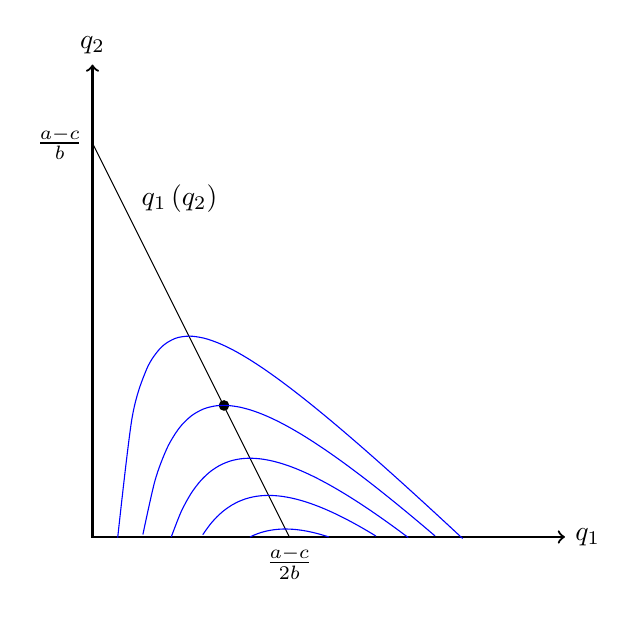
\begin{tikzpicture}[scale=1]
    \draw [thick,<->] (0,6) node [above] {$q_2$} --(0,0)--(6,0) node [right] {$q_1$};
    \node [above right] at (0.5,4) {$q_1\left( q_2 \right)$};
    \draw (0,5)--(2.5,0);
    \draw[fill] (1.67,1.67) circle [radius =0.06];
    \draw[domain=2:3,smooth,variable=\x,blue] plot ({\x},{5-\x-6/\x});
    \draw[domain=1.4:3.6,smooth,variable=\x,blue] plot ({\x},{5-\x-5/\x});
    \draw[domain=1.00:4.01,smooth,variable=\x,blue] plot ({\x},{5-\x-4/\x});
    \draw[domain=0.64:4.35,smooth,variable=\x,blue] plot ({\x},{5-\x-2.77/\x});
    \draw[domain=0.32:4.7,smooth,variable=\x,blue] plot ({\x},{5-\x-1.5/\x});
    \node [below] at (2.5,0) {$\frac{a-c}{2b}$};
    \node [left] at (0,5) {$\frac{a-c}{b}$};
  \end{tikzpicture}
\end{center}
Isoprofit curves closer to the monopoly profits of $\frac{a-c}{2b}$ give higher profits. For any level of output of firm 2, firm 1 will produce an output to put it on the isoprofit curve with the higher profits. This point is also where the reaction function is: the reaction curve gives the quantity firm 1 should produce to get on the best isoprofit curve, given any output for firm 2. The reaction function joins the maximum of all the isoprofit curves. More specifically, the reaction curves are the loci of maxima of the isoprofit curves for each firm. Firm 2's isoprofit curves are defined in a similar way.
\subsubsection*{Quantity Leadership (Stackelberg)}
Here firm 1 produces its quantity first. Then firm 2 observes this quantity and
decides how much to produce. Firm 2 will produce according to the same reaction
function as in Cournot, $q_2\left( q_1 \right)$. When firm 1 decides on a
quantity to produce, it will internalize firm 2's reaction in its decision as it knows exactly how much firm 2 will produce in response:
\[
  \underset{q_1}{\max}\; p\left( q_1+q_2\left( q_1 \right) \right)q_1 - c\left(
  q_1 \right)
\]
In this case, the leading firm can take advantage of moving first. Let's return to the linear demand and costs example. Firm 1 knows that firm 2's reaction function is:
\[q_2\left( q_1 \right)= \frac{a-c-bq_1}{2b}\]
Therefore we can put this directly in firm 1's profit function:
\begin{align*}
  \pi_1\left( q_1,q_2\left( q_1 \right) \right)=&\left[ a-b\left( q_1+q_2\left( q_1 \right) \right) \right]q_1 - cq_1\\
  =&\left[ a-b\left( q_1+\frac{a-c-bq_1}{2b} \right) \right]q_1 - cq_1\\
  =& aq_1 -bq_1^2 -\frac{a-c}{2}q_1+\frac{bq_1^2}{2} - cq_1\\
  =& \frac{a-c}{2}q_1-\frac{bq_1^2}{2}
\end{align*}
Firm 1 will maximize this profit function by taking the derivative with respect to $q_1$ and setting it equal to zero:
\[
  \frac{d\pi_1}{dq_1}=\frac{a-c}{2}-bq_1 = 0 \;\;\;\Longrightarrow \;\;\;
  q_1=\frac{a-c}{2b}
\]
This turns out to be the monopoly quantity. Firm 2 will respond to this by producing according to its reaction function:
\[
  q_2\left( q_1 \right)= \frac{a-c-bq_1}{2b} = \frac{a-c-b\frac{a-c}{2b}}{2b}=\frac{\frac{a-c}{2}}{2b}=\frac{a-c}{4b}
\]
Graphically, firm 1 will choose the quantity on firm 2's reaction function
which puts it on its highest isoprofit curve. This will be the isoprofit curve that ``just touches'' firm 2's reaction curve:
\begin{center}
  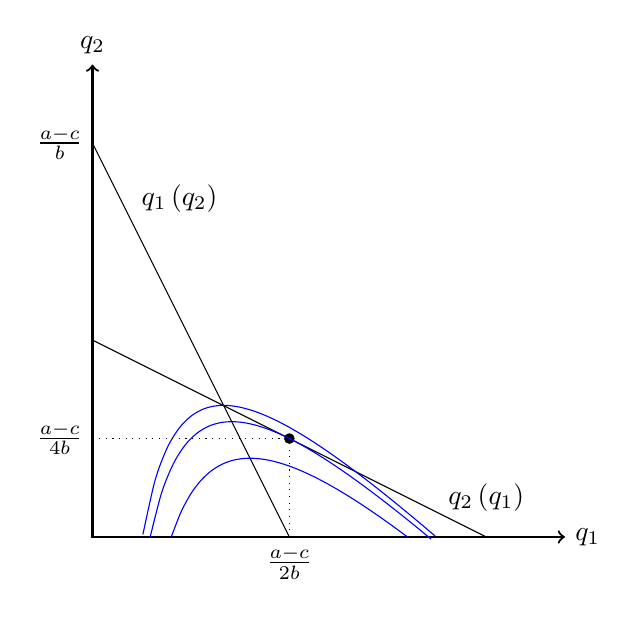
\begin{tikzpicture}[scale=1]
    \draw [thick,<->] (0,6) node [above] {$q_2$} --(0,0)--(6,0) node [right] {$q_1$};
    \node [above right] at (0.5,4) {$q_1\left( q_2 \right)$};
    \node [above] at (5,0.2) {$q_2\left( q_1 \right)$};
    \draw (0,5)--(2.5,0);
    \draw (0,2.5)--(5,0);
    \draw[fill] (2.5,1.25) circle [radius =0.06];
    \draw[domain=0.64:4.35,smooth,variable=\x,blue] plot ({\x},{5-\x-2.77/\x});
    \draw[domain=0.73:4.30,smooth,variable=\x,blue] plot ({\x},{5-\x-3.125/\x});
    \draw[domain=1.00:4.01,smooth,variable=\x,blue] plot ({\x},{5-\x-4/\x});
    \node [below] at (2.5,0) {$\frac{a-c}{2b}$};
    \draw [dotted] (2.5,0) -- (2.5, 1.25);
    \draw [dotted] (0,1.25) -- (2.5, 1.25);
    \node [left] at (0,1.25) {$\frac{a-c}{4b}$};
    \node [left] at (0,5) {$\frac{a-c}{b}$};
  \end{tikzpicture}
\end{center}
The total quantity produced in Stackelberg oligopoly is $\frac{a-c}{2b}+\frac{a-c}{4b}=\frac{3\left( a-c \right)}{4b}$, which is higher than under Cournot.
We can compare each of the models' total outputs with perfect competition and monopoly:
\begin{itemize}
  \item In perfect competition, total industry output is $\frac{a-c}{b}$.
  \item In monopoly, the monopolist produces $\frac{1}{2}\frac{a-c}{b}$.
  \item In Cournot, each firm produces $\frac{1}{3}\frac{a-c}{b}$ so in total we have $\frac{2}{3}\frac{a-c}{b}$.
  \item In Stackelberg, the leader produces $\frac{1}{2}\frac{a-c}{b}$ and the follower produces $\frac{1}{4}\frac{a-c}{b}$ so in total we have $\frac{3}{4}\frac{a-c}{b}$.
\end{itemize}
\section{Oligopoly Collusion}
Collusion is went competing firms decide to coordinate to maximize their joint profits. If firms in Cournot competition want to collude, they should jointly maximize the sum of profits:
\[
  \underset{q_1,q_2}{\max}\; p\left( q_1+q_2 \right)q_1-c\left( q_1 \right) +p\left( q_1+q_2 \right)q_2 -c\left( q_2 \right)
\]
Let's use the linear demand and cost example again from before. Here, the firms' joint maximization problem is:
\[
\underset{q_1,q_2}{\max}\; \left[ a-b\left( q_1+q_2 \right) \right]q_1-cq_1+\left[ a-b\left( q_1+q_2 \right) \right]q_2 -cq_2
\]
Using $q=q_1+q_2$, this is:
\[
  \pi\left( q \right)= \left( a-bq \right)q - cq = \left( a-c \right)q-bq^2
\]
This is the same as the monopoly problem. The firms will jointly produce $q=\frac{a-c}{2b}$ and will jointly earn the monopoly profits. Each will individually produce $q_1=q_2=\frac{a-c}{4b}$, half the monopoly output, and each firm will earn profits $\pi_{cartel}=\frac{\left( a-c \right)^2}{8b}$, half the monopoly profits.

In Cournot competition, each firm earns profits $\pi_{Cournot}=\frac{\left( a-c
\right)^2}{9b}$, so profits under collusion are higher.
\subsubsection*{Cheating on the Cartel}
A firm will be tempted to cheat on the cartel because it is producing a quantity that is not on its reaction function. It can achieve a higher profit by producing the quantity according to its reaction function, provided the other firm doesn't change its output.

In the linear demand and costs example, firm 1's reaction
function is $q_1\left( q_2 \right)=\frac{1}{2b}\left( a-c-bq_2 \right)$. If firm 2 is producing the cartel quantity, $q_2=\frac{a-c}{4b}$, firm 1 will
want to cheat and produce:
\[
  q_1=\frac{1}{2b}\left( a-c-bq_2 \right)=\frac{1}{2b}\left( a-c-b\left( \frac{a-c}{4b} \right) \right)=\frac{1}{2b}\left( 3\left( \frac{a-c}{4} \right) \right)=\frac{3}{8}\frac{a-c}{b}
\]
This will earn the cheating firm profits:
\[\pi_{cheat}=\left( a-c \right)q_1-bq_1^2-bq_1q_2=
  \frac{3}{8}\frac{\left( a-c \right)^2}{b}- \frac{9}{64} \frac{\left( a-c \right)^2}{b}-\frac{3}{8}\times \frac{1}{4}\frac{\left( a-c \right)^2}{b}=
  \frac{9}{64}\frac{\left( a-c \right)^2}{b}
\]
This is provided firm 2 continues producing at the cartel quantity. So:
\[
  \pi_{cheat}>\pi_{cartel}>\pi_{Cournot}
\]
The cartel is not stable as both firms will want to cheat. Graphically, firm 1 will move the its reaction function where firm 2 continues to produce the cartel quantity of $\frac{a-c}{4b}$. This is at $\frac{3}{8}\frac{a-c}{b}$. This brings firm 1 onto a better isoprofit curve.
\begin{center}
  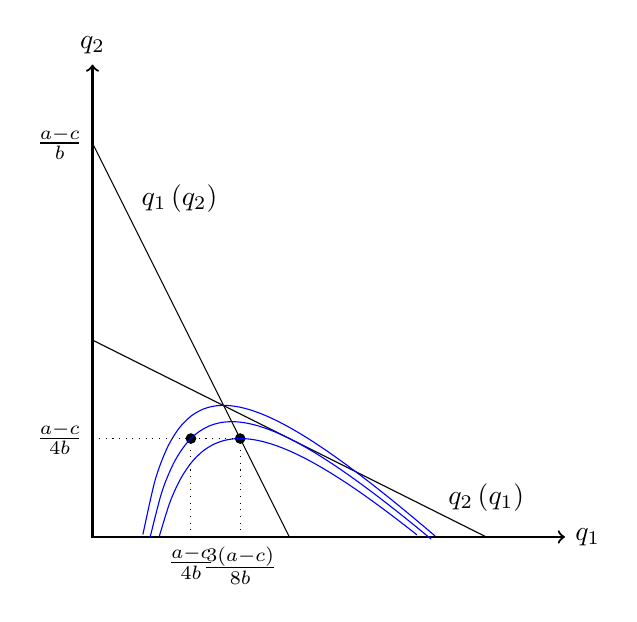
\begin{tikzpicture}[scale=1]
    \draw [thick,<->] (0,6) node [above] {$q_2$} --(0,0)--(6,0) node [right] {$q_1$};
    \node [above right] at (0.5,4) {$q_1\left( q_2 \right)$};
    \node [above] at (5,0.2) {$q_2\left( q_1 \right)$};
    \draw (0,5)--(2.5,0);
    \draw (0,2.5)--(5,0);
    \draw[fill] (1.25,1.25) circle [radius =0.06];
    \draw[fill] (1.875,1.25) circle [radius =0.06];
    \draw[domain=0.64:4.35,smooth,variable=\x,blue] plot ({\x},{5-\x-2.77/\x});
    \draw[domain=0.73:4.30,smooth,variable=\x,blue] plot ({\x},{5-\x-3.125/\x});
    \draw[domain=0.85:4.12,smooth,variable=\x,blue] plot ({\x},{5-\x-3.5156/\x});
    \node [below] at (1.25,0) {$\frac{a-c}{4b}$};
    \draw [dotted] (1.875,0) -- (1.875, 1.25);
    \draw [dotted] (1.25,0) -- (1.25, 1.25);
    \draw [dotted] (0,1.25) -- (1.875, 1.25);
    \node [left] at (0,1.25) {$\frac{a-c}{4b}$};
    \node [below] at (1.875,0) {$\frac{3\left(a-c\right)}{8b}$};
    \node [left] at (0,5) {$\frac{a-c}{b}$};
  \end{tikzpicture}
\end{center}
\subsubsection*{Maintaining a Cartel}
The firms might be able to sustain the cartel if the firms decided that if one firm cheated on the cartel, they would both play at the Cournot equilibrium forever after. This would work if the interest rate/discount rate, $r$, is not too large.
\begin{itemize}
  \item The present value from staying in the cartel forever (cartel profits today plus cartel profits forever after): $\pi_{cartel}+\frac{\pi_{cartel}}{r}= \frac{\left( 1+r \right)}{r}\pi_{cartel}$
  \item The present value from cheating today and getting Cournot profits forever after:
    $\pi_{cheat}+\frac{\pi_{Cournot}}{r}$
  \item Provided $\frac{\left( 1+r \right)}{r}\pi_{cartel}> \pi_{cheat}+\frac{\pi_{Cournot}}{r}$, the cartel will be stable.
\end{itemize}
With our example of linear demand and costs we hvae $\pi_{cartel}=\frac{\left( a-c \right)^2}{8b}$, $\pi_{Cournot}=\frac{\left( a-c \right)^2}{9b}$ and $\pi_{cheat}=\frac{9\left( a-c \right)^2}{64b}$. The cartel is stable if:
\[\left( \frac{1+r}{r} \right)\frac{\left( a-c \right)^2}{8b} > \frac{9\left( a-c \right)^2}{64b} +\frac{\left( a-c \right)^2}{9br}\;\;\; \Longrightarrow \;\;\; \frac{1+r}{8r}>\frac{9}{64}+\frac{1}{9r}
\]
The cartel is stable in this case if $r<0.88$. At a very high interest rate, the firm will want to cheat on the cartel.




\end{document}
